% Supplementary Information for the EMSE 2026 Agentic SE submission.
% Tables are generated from validated analysis outputs.
\documentclass[pdflatex,sn-basic]{sn-jnl}

\usepackage{graphicx}
\usepackage{amsmath,amssymb}
\usepackage{booktabs}
\usepackage{longtable}
\usepackage{tabularx}
\usepackage{xurl}
\usepackage{placeins}
\usepackage{needspace}
% Table cells carry identifiers such as pr_review_comments, which must not
% be hyphenated across lines.
\newcolumntype{L}[1]{>{\raggedright\arraybackslash\hyphenpenalty=10000%
\exhyphenpenalty=10000}p{#1}}
\newcolumntype{Y}{>{\raggedright\arraybackslash}X}
% sn-jnl does not define \tableofcontents or \listoftables, but it keeps the
% kernel entry writers and the \l@section, \l@subsection, and \l@table entry
% formats. These two commands only reopen the standard listing files.
\makeatletter
\newcommand{\snlcontents}{\section*{Contents}\@starttoc{toc}}
\newcommand{\snllistoftables}{\section*{List of tables}\@starttoc{lot}}
\makeatother
\raggedbottom
\setlength{\bibsep}{0.25em}

\begin{document}

\title[Online Resource 1]{Online Resource 1: Supplementary Information for ``Participation Is Not Collaboration: Tracing Public Ownership After Cross-Product Agent Review''}

\author*[1]{\fnm{Dao Sy Duy} \sur{Minh}}\email{Corresponding email pending}
\author[1]{\fnm{Huynh Trung} \sur{Kiet}}
\author[1]{\fnm{Tran Chi} \sur{Nguyen}}
\author[1]{\fnm{Pham Phu} \sur{Hoa}}
\author[1]{\fnm{Nguyen Lam Phu} \sur{Quy}}
\affil*[1]{\orgdiv{Affiliation pending}, \orgname{Institution pending},
  \orgaddress{\city{City pending}, \country{Country pending}}}

\abstract{This appendix gives the complete data contracts, joins, cohort rules,
estimands, robustness checks, falsification tests, and experiment decisions for
the accompanying article. It separates observed GitHub events from derived
labels and keeps semantic and causal claims outside the evidence available in
the public trace. All reported tables are generated from the validated analysis
outputs rather than typed independently.}

\keywords{coding agents, multi-agent software engineering, code review, supplementary information, reproducibility}
\maketitle

\noindent\textbf{Journal:} Empirical Software Engineering\qquad
\textbf{File:} Online Resource 1

\snlcontents

\clearpage

\section*{Where to find what}

Each row names a claim in the main article and the appendix table that carries
the numbers behind it. Sections~\ref{app:rq1} to \ref{app:rq4} explain how each
table was built.

\begingroup
\small
\setlength{\tabcolsep}{4pt}
\noindent\begin{tabularx}{\textwidth}{@{}Y c c@{}}
\toprule
Claim or question & Table & Page \\
\midrule
\multicolumn{3}{@{}l}{\textit{RQ1 -- is there a handoff?}} \\
Participation funnel; fewer than 1\% of trigger PRs carry a different-product exact reply & \ref{tab:s-cohort} & \pageref{tab:s-cohort} \\
First public owner after each burst window, including the 53\% user against 19\% mapped-product split at five minutes & \ref{tab:s-burst} & \pageref{tab:s-burst} \\
Tied first timestamps, the fixed priority order, every leave-one-out exclusion, and the order placebos that reject the escalation and persistence stories & \ref{tab:s-rq1-robustness} & \pageref{tab:s-rq1-robustness} \\
\addlinespace
\multicolumn{3}{@{}l}{\textit{RQ2 -- who bridges the boundary?}} \\
13.4-point matched gap in later visible action across the product boundary, and the seven in ten first user bridges who had already reviewed in the repository & \ref{tab:s-rq2} & \pageref{tab:s-rq2} \\
\addlinespace
\multicolumn{3}{@{}l}{\textit{RQ3 -- who writes the connection, and does it mark a later state?}} \\
17.3-point addressed-edge contrast, reply windows, repository fixed effects, product-pair drops, specificity control, and the four-state 48-hour gradient & \ref{tab:s-addressed-edge} & \pageref{tab:s-addressed-edge} \\
Landmark selection, who writes the edge, stricter edge rules, pre-trigger balance, the E-value of 2.27, tipping grid, negative controls, the conditional shuffle test at $p=0.007$, and the whole-population hazard near 1.7 & \ref{tab:s-sensitivity} & \pageref{tab:s-sensitivity} \\
\addlinespace
\multicolumn{3}{@{}l}{\textit{RQ4 -- what makes someone answer across the boundary?}} \\
Issue link and answered review points, by reviewer relation, with the shuffled-label check & \ref{tab:s-task-context} & \pageref{tab:s-task-context} \\
\addlinespace
\multicolumn{3}{@{}l}{\textit{Measurement contract used by all four questions}} \\
Release layers, units, and event-table coverage & \ref{tab:s-dataset} & \pageref{tab:s-dataset} \\
Exact account allowlist and the code-level glossary & \ref{tab:s-definitions} & \pageref{tab:s-definitions} \\
Named estimation specifications, their formulas, and every resampling setting & \ref{tab:s-specifications} & \pageref{tab:s-specifications} \\
Data-quality and temporal gates, with column-by-column leakage tags & \ref{tab:s-quality} & \pageref{tab:s-quality} \\
\addlinespace
\multicolumn{3}{@{}l}{\textit{Negative results, external checks, and reproduction}} \\
Structural same-locus overlap, still semantically uncoded, and the external evidence ladder with its failed replication gate & \ref{tab:s-external} & \pageref{tab:s-external} \\
Ordered run contract with frozen row counts, and every kept, relocated, or rejected result & \ref{tab:s-record} & \pageref{tab:s-record} \\
\bottomrule
\end{tabularx}
\endgroup

\snllistoftables

\clearpage

\section{Purpose, evidence levels, and the interpretation boundary}\label{app:purpose}

The main article keeps only the numbers needed to follow the story. This
appendix carries the complete measurement and sensitivity record, and every
table in it is generated from the validated analysis products rather than typed
by hand.

\subsection{Four evidence levels}\label{app:levels}

\emph{Product presence} means that two mapped products appear on one pull
request (PR). An \emph{addressed edge} requires a reply whose parent identifier
is the exact cross-product trigger. A \emph{next owner} is the first public
actor class after a declared rapid-burst window. A \emph{later state} is
measured only after a fixed landmark. These levels must not be collapsed into a
single ``multi-agent'' indicator.

\subsection{The interpretation boundary}\label{app:boundary}

This subsection states every caveat that holds for every number in this
appendix. Later sections do not restate it; they cross-reference it and add
only what is specific to their own analysis.

The study observes public GitHub accounts and events, and nothing else. A
mapped product label does not reveal its foundation model, its private
messages, or its internal run boundary. A GitHub \texttt{User} account does not
prove unaided manual work. A later event does not prove that a review point was
understood or fixed. An answered review point is not a resolved one. Public
product presence is not private communication. Temporal succession is not
semantic response. Account history is not verified memory retrieval. A
force-push is visible branch movement, not a verified repair. Merge is an
integration state, not code quality.

Every outcome model in this paper is therefore an observational association.
None of them identifies an intervention. Every outcome model is also a linear
probability model, which can predict outside the unit interval. Task difficulty,
maintainer intent, review meaning, and private activity are not measured, and
any of them can select both the public topology and the later state.
Section~\ref{app:bounds} bounds how much unmeasured structure would be needed to
remove the main association; it does not convert that association into an
effect. These boundaries are part of the result, not only limitations.

This boundary also separates the study from prior work on cross-product review
prevalence, broad reviewer-type sequences, and developer response
\citep{selvanayagam2026a2a,zhong2026agenticreview,cynthia2026responses}.
Those studies motivate the narrower event-level checks reported here.

\section{Dataset release, grain, and joins}\label{app:data}

\begin{figure}[htbp]
\centering
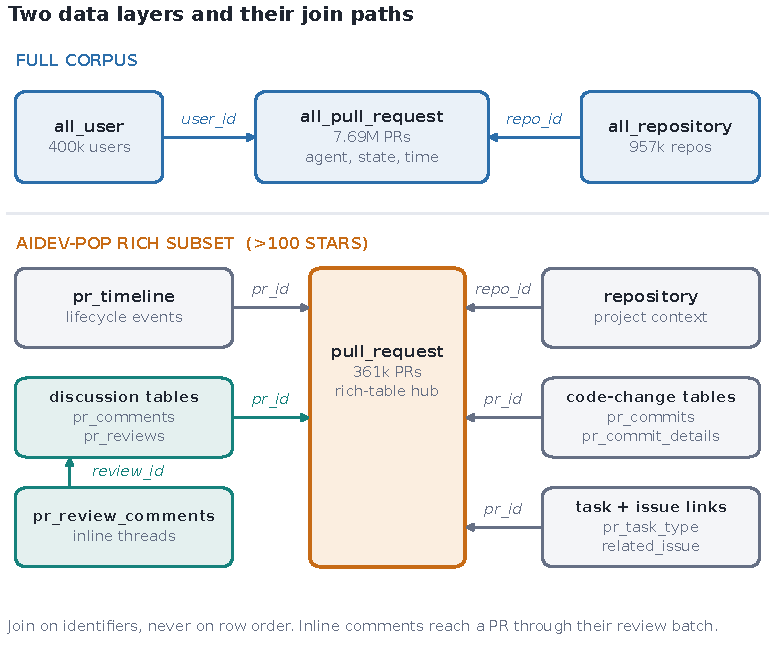
\includegraphics[width=\linewidth]{FigS1.pdf}
\caption{AIDev release layers and the identifier paths used in this study.
The full corpus supports broad PR, repository, and account checks. The rich
layer supports event-level analysis. Inline review comments reach a PR through
their submitted-review identifier; row order is never a join key.}
\label{fig:s-schema}
\end{figure}

The analysis pins AIDev-7.6M at revision
\nolinkurl{37bbe1533e26cc1e1374917dba1186d1c8a4dc81}. The full release is used
for corpus checks. Interaction analyses use AIDev-pop, the rich layer for
repositories with more than 100 stars. Table~\ref{tab:s-dataset} reports the
release profile in its first block and event-table coverage in its second.

The PR table is the hub. Submitted reviews join directly by PR identifier.
Inline review comments do not contain a PR identifier, so they first join to a
submitted review by \texttt{pull\_request\_review\_id}; the review then joins to
the PR. All inline-review identifiers used in this join resolve. PR comments
and timeline events join directly to the PR. Commit-detail rows have one row per
file and commit; any PR-level commit count must deduplicate commit SHA values
before aggregation.

Figure~\ref{fig:s-coverage} shows why each analysis declares its own
denominator: rich tables cover different subsets of the same PR backbone.

\begin{figure}[htbp]
\centering
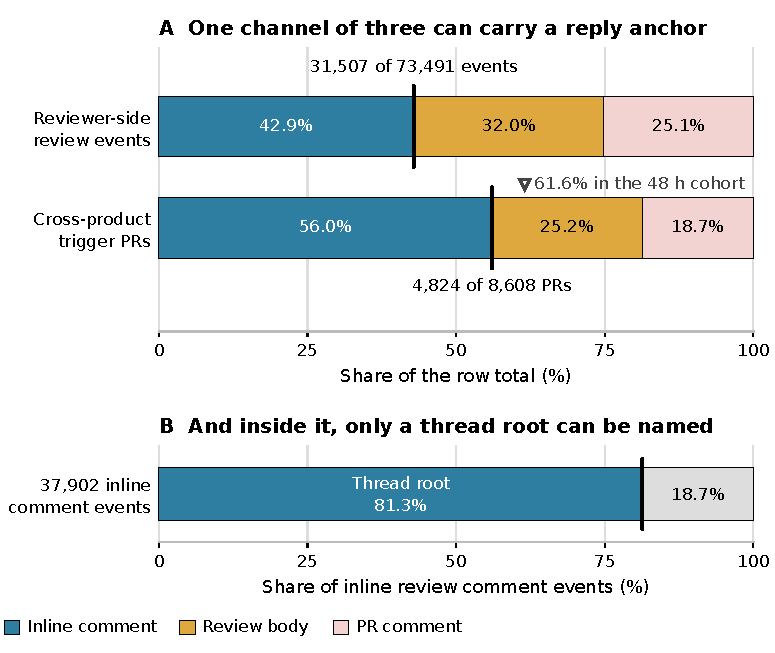
\includegraphics[width=\linewidth]{FigS2.pdf}
\caption{Availability of rich feature groups across the 361,296-PR backbone.
Coverage is not uniform and missing linked rows are not assumed to be negative
events. Each model therefore uses a declared feature-specific denominator.}
\label{fig:s-coverage}
\end{figure}
\FloatBarrier

% Generated deterministically; do not edit this file by hand.

\FloatBarrier
\needspace{8\baselineskip}
\begingroup
\footnotesize
\setlength{\tabcolsep}{3pt}
\begin{longtable}{@{}L{0.12\textwidth}L{0.20\textwidth}L{0.07\textwidth}L{0.13\textwidth}L{0.09\textwidth}L{0.31\textwidth}@{}}
\caption{Release inventory, units, analytical roles, and event-table coverage.}\label{tab:s-dataset}\\
\toprule
Block & Table or feature group & Scope & Unit & Rows & Fields, coverage, and role \\
\midrule
\endfirsthead
\caption*{Release inventory, units, analytical roles, and event-table coverage. (continued)}\\
\toprule
Block & Table or feature group & Scope & Unit & Rows & Fields, coverage, and role \\
\midrule
\endhead
Release inventory & \nolinkurl{all_pull_request} & Full corpus & One pull request & 7,685,281 & 14 fields; PR identity, agent, author, state, timestamps, and repository \\
Release inventory & \nolinkurl{all_repository} & Full corpus & One repository & 957,209 & 8 fields; Repository name, language, license, fork status, stars, and forks \\
Release inventory & \nolinkurl{all_user} & Full corpus & One GitHub user & 399,962 & 5 fields; Contributor account age and follower/following counts \\
Release inventory & \nolinkurl{pull_request} & Rich layer & One pull request & 361,296 & 14 fields; PR backbone for the richer event and content tables \\
Release inventory & \nolinkurl{repository} & Rich layer & One repository & 25,402 & 8 fields; Repository context for the richer subset \\
Release inventory & \nolinkurl{pr_timeline} & Rich layer & One PR timeline event & 3,018,358 & 8 fields; Review, assignment, label, closure, and other lifecycle events \\
Release inventory & \nolinkurl{pr_comments} & Rich layer & One issue-style PR comment & 373,549 & 7 fields; Conversation text, actor, actor type, and time \\
Release inventory & \nolinkurl{pr_reviews} & Rich layer & One submitted PR review & 281,170 & 8 fields; Review decision, reviewer type, text, and submission time \\
Release inventory & \nolinkurl{pr_review_comments} & Rich layer & One inline review comment & 289,780 & 15 fields; Inline discussion tied to a file and diff position \\
Release inventory & \nolinkurl{pr_commits} & Rich layer & One commit attached to a PR & 718,779 & 5 fields; Commit author, committer, SHA, and message \\
Release inventory & \nolinkurl{pr_commit_details} & Rich layer & One changed file within a PR commit & 6,112,623 & 14 fields; Change size, filename, file status, and patch text \\
Release inventory & \nolinkurl{pr_task_type} & Rich layer & One classified pull request & 32,702 & 17 fields; Task type, model reason, and classification confidence \\
Release inventory & \nolinkurl{issue} & Rich layer & One linked issue & 29,111 & 9 fields; Issue title, body, author, state, and timestamps \\
Release inventory & \nolinkurl{related_issue} & Rich layer & One PR-issue link & 38,006 & 3 fields; Bridge between PRs and issues, with link source \\
PR coverage & Timeline events & Rich layer & Linked event or feature rows & 3,018,358 & 197,471 matched PRs; 54.66\% PR coverage; 0 orphan PR IDs \\
PR coverage & File-level changes & Rich layer & Linked event or feature rows & 6,112,623 & 197,330 matched PRs; 54.62\% PR coverage; 0 orphan PR IDs \\
PR coverage & Commits & Rich layer & Linked event or feature rows & 718,779 & 197,335 matched PRs; 54.62\% PR coverage; 0 orphan PR IDs \\
PR coverage & Conversation comments & Rich layer & Linked event or feature rows & 373,549 & 110,011 matched PRs; 30.45\% PR coverage; 0 orphan PR IDs \\
PR coverage & Submitted reviews & Rich layer & Linked event or feature rows & 281,170 & 83,081 matched PRs; 23.00\% PR coverage; 0 orphan PR IDs \\
PR coverage & Inline review comments & Rich layer & Linked event or feature rows & 289,780 & 47,251 matched PRs; 13.08\% PR coverage; 0 orphan PR IDs \\
PR coverage & Task classification & Rich layer & Linked event or feature rows & 32,702 & 32,702 matched PRs; 9.05\% PR coverage; 0 orphan PR IDs \\
PR coverage & Linked issues & Rich layer & Linked event or feature rows & 38,006 & 28,987 matched PRs; 8.02\% PR coverage; 0 orphan PR IDs \\
\bottomrule
\end{longtable}
\noindent\footnotesize \textit{Note:} The rich layer contains repositories with more than 100 stars. Inventory row counts come from Parquet metadata, so large content tables are not expanded in memory. The coverage block describes the 361,296 AIDev-pop pull requests: coverage means that a pull request has at least one linked row, and inline comments resolve through their submitted-review identifier before joining to the pull request.
\endgroup

\FloatBarrier

\section{Identity registry, trigger construction, and glossary}\label{app:identity}

\subsection{Allowlist and trigger rule}\label{app:allowlist}

Product attribution uses an allowlist of exact vendor-controlled GitHub
identities, given in full in Table~\ref{tab:s-definitions}, Panel A. Similar
names and
unknown bots are not guessed. The unit for the main cohort is one PR with its
first mapped feedback event written by a product different from the agent label
attributed to the PR author.

Eligible feedback sources are a submitted review, an inline review comment, or
a PR comment. The event must be after PR creation and no later than PR closure.
The common observation boundary is 15 April 2026 at 00:00 UTC. PR creation is
cut off on 31 March 2026, which leaves time to observe follow-up events.

If the inline trigger belongs to a submitted review, the enclosing review is the
same batch and is not counted as a later review. A later review needs a
different review-batch identifier. These rules prevent one API batch from
answering itself.

\subsection{What the reply identifier points at}\label{app:reply-target}

For an inline trigger, a direct reply must carry the trigger's own comment
identifier as its reply target. A reply elsewhere on the PR does not count.

GitHub sets that target to the first comment of an inline thread rather than to
the immediately preceding comment, and the pinned release behaves the same way:
of 88,907 inline replies, none names a comment that is itself a reply. Reply
threads are therefore one level deep, and the construct is precisely ``a reply
in the thread the trigger opened''. Two consequences are measured rather than
assumed. The exposure is structurally impossible when the trigger sits
mid-thread, which happens for 13 of 3,526 cross-product inline triggers and for
3 of the 1,067 landmark PRs, none of the latter exposed; for same-product
triggers it happens in 46\% of cases, which is a further reason the two rates
are not directly comparable. And within a multi-reply thread a later reply may
answer an earlier reply instead of the trigger: 92 of the 109 exposed PRs carry
exactly one reply in the thread, 15 carry two, and two carry more.

\subsection{Glossary of load-bearing terms}\label{app:glossary}

Several short terms carry weight across all four research questions, so
Table~\ref{tab:s-definitions}, Panel B, states each one as the rule the code
applies. It
covers a decisive review, branch movement, the residual untyped class, the five
mutually exclusive actor states, the seven response actor roles, and the
automation episode with its five-minute gap parameter. Each definition was read
back from the analysis code rather than restated from the article. The table
does not say how often each label occurs, and it says nothing about what a
labelled event meant to the people or products involved.

% Generated deterministically; do not edit this file by hand.

\FloatBarrier
\needspace{8\baselineskip}
\begingroup
\footnotesize
\setlength{\tabcolsep}{3pt}
\begin{longtable}{@{}L{0.22\textwidth}L{0.57\textwidth}L{0.17\textwidth}@{}}
\caption{Attribution allowlist and the glossary of load-bearing terms.}\label{tab:s-definitions}\\
\endfirsthead
\caption*{Attribution allowlist and the glossary of load-bearing terms. (continued)}\\
\endhead
\toprule
\multicolumn{3}{@{}l}{\textbf{Panel A. Attribution allowlist}} \\
\midrule
Mapped product & Exact GitHub login(s), matched case-insensitively &  \\
\midrule
\texttt{Claude\_Code} & \texttt{claude[bot]} &  \\
\texttt{Copilot} & \texttt{copilot}, \texttt{copilot-pull-request-reviewer[bot]}, \texttt{copilot-swe-agent[bot]} &  \\
\texttt{Cursor} & \texttt{cursor[bot]} &  \\
\texttt{Devin} & \texttt{devin-ai-integration[bot]} &  \\
\texttt{Google\_Jules} & \texttt{google-labs-jules[bot]} &  \\
\texttt{OpenAI\_Codex} & \texttt{chatgpt-codex-connector[bot]} &  \\
\midrule
\multicolumn{3}{@{}l}{\textbf{Panel B. Glossary of load-bearing terms}} \\
\midrule
Term & Definition in the code & Where it is defined \\
\midrule
Decisive review & A submitted review whose state is APPROVED or CHANGES\_REQUESTED. Commented and pending reviews are not decisive. & Landmark cohort builder \\
Branch movement & A \texttt{head\_ref\_force\_pushed} timeline event on the PR. It is visible movement of the branch, not a verified repair. & Timeline event filter \\
Untyped activity & A post-trigger event row that is not a user account, a mapped product, or another bot. It is the residual class and is always reported together with branch movement. & First-state classifier \\
State: user account & The event's GitHub user type is User. User evidence takes precedence over product mapping. & First-state classifier \\
State: mapped product & The event is not a User event and its account is on the six-product allowlist. & First-state classifier \\
State: other bot & The event's user type is Bot and the account is not on the allowlist. & First-state classifier \\
State: branch movement or untyped activity & Every remaining event row, which in this release is branch movement and untyped rows. & First-state classifier \\
State: no later action within seven days & No post-burst event occurs inside the seven-day response window. & First-state classifier \\
Role: the PR author's own user account & A User account whose login equals the PR author's login. & Response actor roles \\
Role: the PR author's product & A mapped product equal to the product attributed to the PR author. & Response actor roles \\
Role: the triggering product & A mapped product equal to the product that wrote the trigger. & Response actor roles \\
Role: a different mapped product & Any other account on the six-product allowlist. & Response actor roles \\
Role: an unmapped bot & A Bot account that is not on the allowlist. & Response actor roles \\
Role: another user account & Any other User account. & Response actor roles \\
Role: unknown actor & An event with no usable user type. The class is kept so that the seven roles stay exhaustive. & Response actor roles \\
Automation episode & A run of post-burst events on one PR in which each event follows the previous one by no more than the gap parameter; a larger gap starts a new episode. The primary gap is five minutes, and the first five minutes after the trigger are excluded before episodes are built. & Episode sessionization \\
Episode state & The highest-priority state inside the episode, using the same priority order as the tie rule. At the five-minute gap, 2,529 of 14,842 episodes mix states. & Episode sessionization \\
\bottomrule
\end{longtable}
\noindent\footnotesize \textit{Note:} Panel A is the exact public-account allowlist used for reviewer-product attribution; logins are matched case-insensitively. Only exact aliases are mapped. Similar names and unknown bots stay outside the six-product registry. Panel B is read from the analysis code: each definition is the rule the code applies, not an interpretation of it. The five states are mutually exclusive and cover every PR at every burst threshold. The seven roles are evaluated in the listed order, so the first matching branch wins. None of these labels reports intent, private activity, or whether a review point was resolved.
\endgroup

\FloatBarrier

\section{Cohorts, denominators, specifications, and uncertainty}\label{app:cohorts}

\subsection{Cohort flow}\label{app:funnel}

Table~\ref{tab:s-cohort}, Panel A, gives the full cohort flow. The seven-day topology
cohort requires a complete observation window and ends earlier if the PR
closes. Exact-parent replies are possible only for inline triggers; therefore
the article reports both the full-cohort and inline-eligible denominators.

The outcome cohort uses a different rule. It first observes public activity for
48 hours after the trigger, retains PRs still open at hour 48, and then observes
merge from hour 48 through day 30. It also requires a complete 30-day outcome
window. This landmark keeps the route definition before the outcome window.

\subsection{Named specifications and resampling settings}\label{app:specifications}

Every outcome model in this paper is a linear probability model fitted by
ordinary least squares, with standard errors clustered on the repository.
Table~\ref{tab:s-specifications} lists each named specification in its first
block: outcome, exposure term, estimator, standard-error type, denominators, and
full model formula. Most formulas are stored with the analysis products
themselves, so the table cannot drift from the fits it describes; the two
ownership-route rows and the two prior-history rows are read back from the
analysis code, which writes no formula column. Reply-window variants at 1, 6,
and 24 hours refit the same formula with that window's exposure term. The table
shows what was fitted and on how many PRs, not that any fit identifies a causal
effect (Section~\ref{app:boundary}).

Uncertainty statements come from two different machines, and the settings are
not uniform, so the second block of the same table lists them per analysis: the
resampling unit, the number of draws, the seed, and the interval method. Cluster
bootstraps resample whole repositories, because PRs in one repository share
policy, integrations, and contributors. The draw count is 10,000 for the matched
contrasts and the same-locus timing share and 5,000 for the burst,
deep-transition, and persistence shares. Order placebos permute event order
inside a PR 500 times. Both randomisation-inference tests permute exposure
labels inside repositories 2,000 times. Every seed derives from one fixed value,
with fixed offsets so that separate quantities do not reuse one draw sequence.
The outcome regressions use no resampling at all. Their intervals come from a
clustered normal approximation, which is why the exact-edge estimate is checked
by permutation as well. Main ordering statements are also recomputed after
removing each repository and each author--reviewer product pair, as reported in
Section~\ref{app:ordering}.

% Generated deterministically; do not edit this file by hand.

\FloatBarrier
\needspace{8\baselineskip}
\begingroup
\footnotesize
\setlength{\tabcolsep}{3pt}
\begin{longtable}{@{}L{0.21\textwidth}L{0.07\textwidth}L{0.18\textwidth}L{0.09\textwidth}L{0.14\textwidth}L{0.23\textwidth}@{}}
\caption{Cohort funnel and the 48-hour ownership routes.}\label{tab:s-cohort}\\
\endfirsthead
\caption*{Cohort funnel and the 48-hour ownership routes. (continued)}\\
\endhead
\toprule
\multicolumn{6}{@{}l}{\textbf{Panel A. Participation-to-addressed-edge denominator funnel}} \\
\midrule
Stage & PRs & Denominator & Share (\%) &  &  \\
\midrule
Complete seven-day trigger cohort & 8,608 & Full cohort & 100.0 &  &  \\
Any later visible action & 5,553 & Full cohort & 64.5 &  &  \\
Inline trigger; exact reply is observable & 4,824 & Full cohort & 56.0 &  &  \\
Exact parent reply & 730 & Full cohort & 8.5 &  &  \\
Exact parent reply & 730 & Inline-eligible & 15.1 &  &  \\
Mapped different-product exact reply & 74 & Full cohort & 0.9 &  &  \\
Mapped different-product exact reply & 74 & Inline-eligible & 1.5 &  &  \\
\midrule
\multicolumn{6}{@{}l}{\textbf{Panel B. Forty-eight-hour ownership routes and later integration}} \\
\midrule
Route & PRs & Later merge (\%) & Median first action (h) & Adjusted difference (pp) & Repository-cluster 95\% interval \\
\midrule
Automation, no later user event & 314 & 40.1 & 0.09 & Reference & -- \\
Automation then user & 162 & 54.9 & 0.06 & +12.9 & [+3.0, +22.7] \\
User first & 467 & 50.1 & 0.51 & +6.1 & [-1.7, +13.9] \\
Movement only & 55 & 58.2 & 2.00 & +11.6 & [-6.7, +30.0] \\
Other activity & 76 & 39.5 & 0.06 & -1.5 & [-14.5, +11.6] \\
No observed action & 659 & 32.2 & -- & -9.2 & [-15.9, -2.5] \\
\bottomrule
\end{longtable}
\noindent\footnotesize \textit{Note:} Panel A is the denominator funnel. An exact parent reply is defined only for an inline trigger. The repeated rows make the full-cohort and eligible denominators explicit. Panel B reports the 48-hour ownership routes. The reference is automation with no later user event. Adjustment uses only pre-trigger activity and trigger context. Routes are observed markers, not assigned treatments.
\endgroup


\FloatBarrier
\needspace{8\baselineskip}
\begingroup
\footnotesize
\setlength{\tabcolsep}{3pt}
\begin{longtable}{@{}L{0.16\textwidth}L{0.16\textwidth}L{0.15\textwidth}L{0.08\textwidth}L{0.38\textwidth}@{}}
\caption{Named estimation specifications and the resampling settings behind every reported interval.}\label{tab:s-specifications}\\
\toprule
Analysis & Design & Uncertainty & PRs / repos & Formula or interval method \\
\midrule
\endfirsthead
\caption*{Named estimation specifications and the resampling settings behind every reported interval. (continued)}\\
\toprule
Analysis & Design & Uncertainty & PRs / repos & Formula or interval method \\
\midrule
\endhead
Exact edge, pre-trigger adjusted (primary) & outcome \texttt{m\allowbreak{}e\allowbreak{}r\allowbreak{}g\allowbreak{}e\allowbreak{}d\allowbreak{}\_\allowbreak{}f\allowbreak{}r\allowbreak{}o\allowbreak{}m\allowbreak{}\_\allowbreak{}4\allowbreak{}8\allowbreak{}h\allowbreak{}\_\allowbreak{}t\allowbreak{}o\allowbreak{}\_\allowbreak{}3\allowbreak{}0\allowbreak{}d\allowbreak{}}; exposure \texttt{e\allowbreak{}x\allowbreak{}a\allowbreak{}c\allowbreak{}t\allowbreak{}\_\allowbreak{}p\allowbreak{}a\allowbreak{}r\allowbreak{}e\allowbreak{}n\allowbreak{}t\allowbreak{}\_\allowbreak{}r\allowbreak{}e\allowbreak{}p\allowbreak{}l\allowbreak{}y\allowbreak{}\_\allowbreak{}b\allowbreak{}y\allowbreak{}\_\allowbreak{}4\allowbreak{}8\allowbreak{}h\allowbreak{}} & Linear probability model by OLS; cluster-robust by repository & 1,067 / 469 & \texttt{m\allowbreak{}e\allowbreak{}r\allowbreak{}g\allowbreak{}e\allowbreak{}d\allowbreak{}\_\allowbreak{}f\allowbreak{}r\allowbreak{}o\allowbreak{}m\allowbreak{}\_\allowbreak{}4\allowbreak{}8\allowbreak{}h\allowbreak{}\_\allowbreak{}t\allowbreak{}o\allowbreak{}\_\allowbreak{}3\allowbreak{}0\allowbreak{}d\allowbreak{} \textasciitilde{}\allowbreak{} e\allowbreak{}x\allowbreak{}a\allowbreak{}c\allowbreak{}t\allowbreak{}\_\allowbreak{}p\allowbreak{}a\allowbreak{}r\allowbreak{}e\allowbreak{}n\allowbreak{}t\allowbreak{}\_\allowbreak{}r\allowbreak{}e\allowbreak{}p\allowbreak{}l\allowbreak{}y\allowbreak{}\_\allowbreak{}b\allowbreak{}y\allowbreak{}\_\allowbreak{}4\allowbreak{}8\allowbreak{}h\allowbreak{} +\allowbreak{} C\allowbreak{}(\allowbreak{}a\allowbreak{}u\allowbreak{}t\allowbreak{}h\allowbreak{}o\allowbreak{}r\allowbreak{}\_\allowbreak{}a\allowbreak{}g\allowbreak{}e\allowbreak{}n\allowbreak{}t\allowbreak{})\allowbreak{} +\allowbreak{} C\allowbreak{}(\allowbreak{}t\allowbreak{}r\allowbreak{}i\allowbreak{}g\allowbreak{}g\allowbreak{}e\allowbreak{}r\allowbreak{}\_\allowbreak{}r\allowbreak{}e\allowbreak{}v\allowbreak{}i\allowbreak{}e\allowbreak{}w\allowbreak{}e\allowbreak{}r\allowbreak{}\_\allowbreak{}a\allowbreak{}g\allowbreak{}e\allowbreak{}n\allowbreak{}t\allowbreak{})\allowbreak{} +\allowbreak{} C\allowbreak{}(\allowbreak{}t\allowbreak{}r\allowbreak{}i\allowbreak{}g\allowbreak{}g\allowbreak{}e\allowbreak{}r\allowbreak{}\_\allowbreak{}m\allowbreak{}o\allowbreak{}n\allowbreak{}t\allowbreak{}h\allowbreak{})\allowbreak{} +\allowbreak{} l\allowbreak{}o\allowbreak{}g\allowbreak{}1\allowbreak{}p\allowbreak{}\_\allowbreak{}t\allowbreak{}r\allowbreak{}i\allowbreak{}g\allowbreak{}g\allowbreak{}e\allowbreak{}r\allowbreak{}\_\allowbreak{}a\allowbreak{}g\allowbreak{}e\allowbreak{}\_\allowbreak{}h\allowbreak{}o\allowbreak{}u\allowbreak{}r\allowbreak{}s\allowbreak{} +\allowbreak{} l\allowbreak{}o\allowbreak{}g\allowbreak{}1\allowbreak{}p\allowbreak{}\_\allowbreak{}p\allowbreak{}r\allowbreak{}e\allowbreak{}\_\allowbreak{}e\allowbreak{}v\allowbreak{}e\allowbreak{}n\allowbreak{}t\allowbreak{}s\allowbreak{} +\allowbreak{} p\allowbreak{}r\allowbreak{}e\allowbreak{}\_\allowbreak{}u\allowbreak{}s\allowbreak{}e\allowbreak{}r\allowbreak{}\_\allowbreak{}e\allowbreak{}v\allowbreak{}e\allowbreak{}n\allowbreak{}t\allowbreak{}s\allowbreak{} +\allowbreak{} p\allowbreak{}r\allowbreak{}e\allowbreak{}\_\allowbreak{}b\allowbreak{}o\allowbreak{}t\allowbreak{}\_\allowbreak{}e\allowbreak{}v\allowbreak{}e\allowbreak{}n\allowbreak{}t\allowbreak{}s\allowbreak{} +\allowbreak{} p\allowbreak{}r\allowbreak{}e\allowbreak{}\_\allowbreak{}d\allowbreak{}e\allowbreak{}c\allowbreak{}i\allowbreak{}s\allowbreak{}i\allowbreak{}v\allowbreak{}e\allowbreak{}\_\allowbreak{}r\allowbreak{}e\allowbreak{}v\allowbreak{}i\allowbreak{}e\allowbreak{}w\allowbreak{}s\allowbreak{} +\allowbreak{} p\allowbreak{}r\allowbreak{}e\allowbreak{}\_\allowbreak{}f\allowbreak{}o\allowbreak{}r\allowbreak{}c\allowbreak{}e\allowbreak{}\_\allowbreak{}p\allowbreak{}u\allowbreak{}s\allowbreak{}h\allowbreak{}e\allowbreak{}s\allowbreak{}} \\
Exact edge, route decomposition (secondary) & outcome \texttt{m\allowbreak{}e\allowbreak{}r\allowbreak{}g\allowbreak{}e\allowbreak{}d\allowbreak{}\_\allowbreak{}f\allowbreak{}r\allowbreak{}o\allowbreak{}m\allowbreak{}\_\allowbreak{}4\allowbreak{}8\allowbreak{}h\allowbreak{}\_\allowbreak{}t\allowbreak{}o\allowbreak{}\_\allowbreak{}3\allowbreak{}0\allowbreak{}d\allowbreak{}}; exposure \texttt{e\allowbreak{}x\allowbreak{}a\allowbreak{}c\allowbreak{}t\allowbreak{}\_\allowbreak{}p\allowbreak{}a\allowbreak{}r\allowbreak{}e\allowbreak{}n\allowbreak{}t\allowbreak{}\_\allowbreak{}r\allowbreak{}e\allowbreak{}p\allowbreak{}l\allowbreak{}y\allowbreak{}\_\allowbreak{}b\allowbreak{}y\allowbreak{}\_\allowbreak{}4\allowbreak{}8\allowbreak{}h\allowbreak{}} & Linear probability model by OLS; cluster-robust by repository & 1,067 / 469 & \texttt{m\allowbreak{}e\allowbreak{}r\allowbreak{}g\allowbreak{}e\allowbreak{}d\allowbreak{}\_\allowbreak{}f\allowbreak{}r\allowbreak{}o\allowbreak{}m\allowbreak{}\_\allowbreak{}4\allowbreak{}8\allowbreak{}h\allowbreak{}\_\allowbreak{}t\allowbreak{}o\allowbreak{}\_\allowbreak{}3\allowbreak{}0\allowbreak{}d\allowbreak{} \textasciitilde{}\allowbreak{} e\allowbreak{}x\allowbreak{}a\allowbreak{}c\allowbreak{}t\allowbreak{}\_\allowbreak{}p\allowbreak{}a\allowbreak{}r\allowbreak{}e\allowbreak{}n\allowbreak{}t\allowbreak{}\_\allowbreak{}r\allowbreak{}e\allowbreak{}p\allowbreak{}l\allowbreak{}y\allowbreak{}\_\allowbreak{}b\allowbreak{}y\allowbreak{}\_\allowbreak{}4\allowbreak{}8\allowbreak{}h\allowbreak{} +\allowbreak{} C\allowbreak{}(\allowbreak{}a\allowbreak{}u\allowbreak{}t\allowbreak{}h\allowbreak{}o\allowbreak{}r\allowbreak{}\_\allowbreak{}a\allowbreak{}g\allowbreak{}e\allowbreak{}n\allowbreak{}t\allowbreak{})\allowbreak{} +\allowbreak{} C\allowbreak{}(\allowbreak{}t\allowbreak{}r\allowbreak{}i\allowbreak{}g\allowbreak{}g\allowbreak{}e\allowbreak{}r\allowbreak{}\_\allowbreak{}r\allowbreak{}e\allowbreak{}v\allowbreak{}i\allowbreak{}e\allowbreak{}w\allowbreak{}e\allowbreak{}r\allowbreak{}\_\allowbreak{}a\allowbreak{}g\allowbreak{}e\allowbreak{}n\allowbreak{}t\allowbreak{})\allowbreak{} +\allowbreak{} C\allowbreak{}(\allowbreak{}t\allowbreak{}r\allowbreak{}i\allowbreak{}g\allowbreak{}g\allowbreak{}e\allowbreak{}r\allowbreak{}\_\allowbreak{}m\allowbreak{}o\allowbreak{}n\allowbreak{}t\allowbreak{}h\allowbreak{})\allowbreak{} +\allowbreak{} l\allowbreak{}o\allowbreak{}g\allowbreak{}1\allowbreak{}p\allowbreak{}\_\allowbreak{}t\allowbreak{}r\allowbreak{}i\allowbreak{}g\allowbreak{}g\allowbreak{}e\allowbreak{}r\allowbreak{}\_\allowbreak{}a\allowbreak{}g\allowbreak{}e\allowbreak{}\_\allowbreak{}h\allowbreak{}o\allowbreak{}u\allowbreak{}r\allowbreak{}s\allowbreak{} +\allowbreak{} l\allowbreak{}o\allowbreak{}g\allowbreak{}1\allowbreak{}p\allowbreak{}\_\allowbreak{}p\allowbreak{}r\allowbreak{}e\allowbreak{}\_\allowbreak{}e\allowbreak{}v\allowbreak{}e\allowbreak{}n\allowbreak{}t\allowbreak{}s\allowbreak{} +\allowbreak{} p\allowbreak{}r\allowbreak{}e\allowbreak{}\_\allowbreak{}u\allowbreak{}s\allowbreak{}e\allowbreak{}r\allowbreak{}\_\allowbreak{}e\allowbreak{}v\allowbreak{}e\allowbreak{}n\allowbreak{}t\allowbreak{}s\allowbreak{} +\allowbreak{} p\allowbreak{}r\allowbreak{}e\allowbreak{}\_\allowbreak{}b\allowbreak{}o\allowbreak{}t\allowbreak{}\_\allowbreak{}e\allowbreak{}v\allowbreak{}e\allowbreak{}n\allowbreak{}t\allowbreak{}s\allowbreak{} +\allowbreak{} p\allowbreak{}r\allowbreak{}e\allowbreak{}\_\allowbreak{}d\allowbreak{}e\allowbreak{}c\allowbreak{}i\allowbreak{}s\allowbreak{}i\allowbreak{}v\allowbreak{}e\allowbreak{}\_\allowbreak{}r\allowbreak{}e\allowbreak{}v\allowbreak{}i\allowbreak{}e\allowbreak{}w\allowbreak{}s\allowbreak{} +\allowbreak{} p\allowbreak{}r\allowbreak{}e\allowbreak{}\_\allowbreak{}f\allowbreak{}o\allowbreak{}r\allowbreak{}c\allowbreak{}e\allowbreak{}\_\allowbreak{}p\allowbreak{}u\allowbreak{}s\allowbreak{}h\allowbreak{}e\allowbreak{}s\allowbreak{} +\allowbreak{} C\allowbreak{}(\allowbreak{}o\allowbreak{}w\allowbreak{}n\allowbreak{}e\allowbreak{}r\allowbreak{}s\allowbreak{}h\allowbreak{}i\allowbreak{}p\allowbreak{}\_\allowbreak{}r\allowbreak{}o\allowbreak{}u\allowbreak{}t\allowbreak{}e\allowbreak{}\_\allowbreak{}4\allowbreak{}8\allowbreak{}h\allowbreak{},\allowbreak{} T\allowbreak{}r\allowbreak{}e\allowbreak{}a\allowbreak{}t\allowbreak{}m\allowbreak{}e\allowbreak{}n\allowbreak{}t\allowbreak{}(\allowbreak{}'\allowbreak{}n\allowbreak{}o\allowbreak{}\_\allowbreak{}o\allowbreak{}b\allowbreak{}s\allowbreak{}e\allowbreak{}r\allowbreak{}v\allowbreak{}e\allowbreak{}d\allowbreak{}\_\allowbreak{}a\allowbreak{}c\allowbreak{}t\allowbreak{}i\allowbreak{}o\allowbreak{}n\allowbreak{}'\allowbreak{})\allowbreak{})\allowbreak{}} \\
Specificity: edge vs non-exact discussion & outcome \texttt{m\allowbreak{}e\allowbreak{}r\allowbreak{}g\allowbreak{}e\allowbreak{}d\allowbreak{}\_\allowbreak{}f\allowbreak{}r\allowbreak{}o\allowbreak{}m\allowbreak{}\_\allowbreak{}4\allowbreak{}8\allowbreak{}h\allowbreak{}\_\allowbreak{}t\allowbreak{}o\allowbreak{}\_\allowbreak{}3\allowbreak{}0\allowbreak{}d\allowbreak{}}; exposure \texttt{e\allowbreak{}x\allowbreak{}a\allowbreak{}c\allowbreak{}t\allowbreak{}\_\allowbreak{}e\allowbreak{}d\allowbreak{}g\allowbreak{}e\allowbreak{}\_\allowbreak{}b\allowbreak{}y\allowbreak{}\_\allowbreak{}4\allowbreak{}8\allowbreak{}h\allowbreak{}} & Linear probability model by OLS; cluster-robust by repository & 615 / 300 & \texttt{m\allowbreak{}e\allowbreak{}r\allowbreak{}g\allowbreak{}e\allowbreak{}d\allowbreak{}\_\allowbreak{}f\allowbreak{}r\allowbreak{}o\allowbreak{}m\allowbreak{}\_\allowbreak{}4\allowbreak{}8\allowbreak{}h\allowbreak{}\_\allowbreak{}t\allowbreak{}o\allowbreak{}\_\allowbreak{}3\allowbreak{}0\allowbreak{}d\allowbreak{} \textasciitilde{}\allowbreak{} e\allowbreak{}x\allowbreak{}a\allowbreak{}c\allowbreak{}t\allowbreak{}\_\allowbreak{}e\allowbreak{}d\allowbreak{}g\allowbreak{}e\allowbreak{}\_\allowbreak{}b\allowbreak{}y\allowbreak{}\_\allowbreak{}4\allowbreak{}8\allowbreak{}h\allowbreak{} +\allowbreak{} C\allowbreak{}(\allowbreak{}a\allowbreak{}u\allowbreak{}t\allowbreak{}h\allowbreak{}o\allowbreak{}r\allowbreak{}\_\allowbreak{}a\allowbreak{}g\allowbreak{}e\allowbreak{}n\allowbreak{}t\allowbreak{})\allowbreak{} +\allowbreak{} C\allowbreak{}(\allowbreak{}t\allowbreak{}r\allowbreak{}i\allowbreak{}g\allowbreak{}g\allowbreak{}e\allowbreak{}r\allowbreak{}\_\allowbreak{}r\allowbreak{}e\allowbreak{}v\allowbreak{}i\allowbreak{}e\allowbreak{}w\allowbreak{}e\allowbreak{}r\allowbreak{}\_\allowbreak{}a\allowbreak{}g\allowbreak{}e\allowbreak{}n\allowbreak{}t\allowbreak{})\allowbreak{} +\allowbreak{} C\allowbreak{}(\allowbreak{}t\allowbreak{}r\allowbreak{}i\allowbreak{}g\allowbreak{}g\allowbreak{}e\allowbreak{}r\allowbreak{}\_\allowbreak{}m\allowbreak{}o\allowbreak{}n\allowbreak{}t\allowbreak{}h\allowbreak{})\allowbreak{} +\allowbreak{} l\allowbreak{}o\allowbreak{}g\allowbreak{}1\allowbreak{}p\allowbreak{}\_\allowbreak{}t\allowbreak{}r\allowbreak{}i\allowbreak{}g\allowbreak{}g\allowbreak{}e\allowbreak{}r\allowbreak{}\_\allowbreak{}a\allowbreak{}g\allowbreak{}e\allowbreak{}\_\allowbreak{}h\allowbreak{}o\allowbreak{}u\allowbreak{}r\allowbreak{}s\allowbreak{} +\allowbreak{} l\allowbreak{}o\allowbreak{}g\allowbreak{}1\allowbreak{}p\allowbreak{}\_\allowbreak{}p\allowbreak{}r\allowbreak{}e\allowbreak{}\_\allowbreak{}e\allowbreak{}v\allowbreak{}e\allowbreak{}n\allowbreak{}t\allowbreak{}s\allowbreak{} +\allowbreak{} p\allowbreak{}r\allowbreak{}e\allowbreak{}\_\allowbreak{}u\allowbreak{}s\allowbreak{}e\allowbreak{}r\allowbreak{}\_\allowbreak{}e\allowbreak{}v\allowbreak{}e\allowbreak{}n\allowbreak{}t\allowbreak{}s\allowbreak{} +\allowbreak{} p\allowbreak{}r\allowbreak{}e\allowbreak{}\_\allowbreak{}b\allowbreak{}o\allowbreak{}t\allowbreak{}\_\allowbreak{}e\allowbreak{}v\allowbreak{}e\allowbreak{}n\allowbreak{}t\allowbreak{}s\allowbreak{} +\allowbreak{} p\allowbreak{}r\allowbreak{}e\allowbreak{}\_\allowbreak{}d\allowbreak{}e\allowbreak{}c\allowbreak{}i\allowbreak{}s\allowbreak{}i\allowbreak{}v\allowbreak{}e\allowbreak{}\_\allowbreak{}r\allowbreak{}e\allowbreak{}v\allowbreak{}i\allowbreak{}e\allowbreak{}w\allowbreak{}s\allowbreak{} +\allowbreak{} p\allowbreak{}r\allowbreak{}e\allowbreak{}\_\allowbreak{}f\allowbreak{}o\allowbreak{}r\allowbreak{}c\allowbreak{}e\allowbreak{}\_\allowbreak{}p\allowbreak{}u\allowbreak{}s\allowbreak{}h\allowbreak{}e\allowbreak{}s\allowbreak{}} \\
Specificity: edge vs any other visible activity & outcome \texttt{m\allowbreak{}e\allowbreak{}r\allowbreak{}g\allowbreak{}e\allowbreak{}d\allowbreak{}\_\allowbreak{}f\allowbreak{}r\allowbreak{}o\allowbreak{}m\allowbreak{}\_\allowbreak{}4\allowbreak{}8\allowbreak{}h\allowbreak{}\_\allowbreak{}t\allowbreak{}o\allowbreak{}\_\allowbreak{}3\allowbreak{}0\allowbreak{}d\allowbreak{}}; exposure \texttt{e\allowbreak{}x\allowbreak{}a\allowbreak{}c\allowbreak{}t\allowbreak{}\_\allowbreak{}e\allowbreak{}d\allowbreak{}g\allowbreak{}e\allowbreak{}\_\allowbreak{}b\allowbreak{}y\allowbreak{}\_\allowbreak{}4\allowbreak{}8\allowbreak{}h\allowbreak{}} & Linear probability model by OLS; cluster-robust by repository & 641 / 309 & \texttt{m\allowbreak{}e\allowbreak{}r\allowbreak{}g\allowbreak{}e\allowbreak{}d\allowbreak{}\_\allowbreak{}f\allowbreak{}r\allowbreak{}o\allowbreak{}m\allowbreak{}\_\allowbreak{}4\allowbreak{}8\allowbreak{}h\allowbreak{}\_\allowbreak{}t\allowbreak{}o\allowbreak{}\_\allowbreak{}3\allowbreak{}0\allowbreak{}d\allowbreak{} \textasciitilde{}\allowbreak{} e\allowbreak{}x\allowbreak{}a\allowbreak{}c\allowbreak{}t\allowbreak{}\_\allowbreak{}e\allowbreak{}d\allowbreak{}g\allowbreak{}e\allowbreak{}\_\allowbreak{}b\allowbreak{}y\allowbreak{}\_\allowbreak{}4\allowbreak{}8\allowbreak{}h\allowbreak{} +\allowbreak{} C\allowbreak{}(\allowbreak{}a\allowbreak{}u\allowbreak{}t\allowbreak{}h\allowbreak{}o\allowbreak{}r\allowbreak{}\_\allowbreak{}a\allowbreak{}g\allowbreak{}e\allowbreak{}n\allowbreak{}t\allowbreak{})\allowbreak{} +\allowbreak{} C\allowbreak{}(\allowbreak{}t\allowbreak{}r\allowbreak{}i\allowbreak{}g\allowbreak{}g\allowbreak{}e\allowbreak{}r\allowbreak{}\_\allowbreak{}r\allowbreak{}e\allowbreak{}v\allowbreak{}i\allowbreak{}e\allowbreak{}w\allowbreak{}e\allowbreak{}r\allowbreak{}\_\allowbreak{}a\allowbreak{}g\allowbreak{}e\allowbreak{}n\allowbreak{}t\allowbreak{})\allowbreak{} +\allowbreak{} C\allowbreak{}(\allowbreak{}t\allowbreak{}r\allowbreak{}i\allowbreak{}g\allowbreak{}g\allowbreak{}e\allowbreak{}r\allowbreak{}\_\allowbreak{}m\allowbreak{}o\allowbreak{}n\allowbreak{}t\allowbreak{}h\allowbreak{})\allowbreak{} +\allowbreak{} l\allowbreak{}o\allowbreak{}g\allowbreak{}1\allowbreak{}p\allowbreak{}\_\allowbreak{}t\allowbreak{}r\allowbreak{}i\allowbreak{}g\allowbreak{}g\allowbreak{}e\allowbreak{}r\allowbreak{}\_\allowbreak{}a\allowbreak{}g\allowbreak{}e\allowbreak{}\_\allowbreak{}h\allowbreak{}o\allowbreak{}u\allowbreak{}r\allowbreak{}s\allowbreak{} +\allowbreak{} l\allowbreak{}o\allowbreak{}g\allowbreak{}1\allowbreak{}p\allowbreak{}\_\allowbreak{}p\allowbreak{}r\allowbreak{}e\allowbreak{}\_\allowbreak{}e\allowbreak{}v\allowbreak{}e\allowbreak{}n\allowbreak{}t\allowbreak{}s\allowbreak{} +\allowbreak{} p\allowbreak{}r\allowbreak{}e\allowbreak{}\_\allowbreak{}u\allowbreak{}s\allowbreak{}e\allowbreak{}r\allowbreak{}\_\allowbreak{}e\allowbreak{}v\allowbreak{}e\allowbreak{}n\allowbreak{}t\allowbreak{}s\allowbreak{} +\allowbreak{} p\allowbreak{}r\allowbreak{}e\allowbreak{}\_\allowbreak{}b\allowbreak{}o\allowbreak{}t\allowbreak{}\_\allowbreak{}e\allowbreak{}v\allowbreak{}e\allowbreak{}n\allowbreak{}t\allowbreak{}s\allowbreak{} +\allowbreak{} p\allowbreak{}r\allowbreak{}e\allowbreak{}\_\allowbreak{}d\allowbreak{}e\allowbreak{}c\allowbreak{}i\allowbreak{}s\allowbreak{}i\allowbreak{}v\allowbreak{}e\allowbreak{}\_\allowbreak{}r\allowbreak{}e\allowbreak{}v\allowbreak{}i\allowbreak{}e\allowbreak{}w\allowbreak{}s\allowbreak{} +\allowbreak{} p\allowbreak{}r\allowbreak{}e\allowbreak{}\_\allowbreak{}f\allowbreak{}o\allowbreak{}r\allowbreak{}c\allowbreak{}e\allowbreak{}\_\allowbreak{}p\allowbreak{}u\allowbreak{}s\allowbreak{}h\allowbreak{}e\allowbreak{}s\allowbreak{}} \\
Specificity: user edge vs non-exact user discussion & outcome \texttt{m\allowbreak{}e\allowbreak{}r\allowbreak{}g\allowbreak{}e\allowbreak{}d\allowbreak{}\_\allowbreak{}f\allowbreak{}r\allowbreak{}o\allowbreak{}m\allowbreak{}\_\allowbreak{}4\allowbreak{}8\allowbreak{}h\allowbreak{}\_\allowbreak{}t\allowbreak{}o\allowbreak{}\_\allowbreak{}3\allowbreak{}0\allowbreak{}d\allowbreak{}}; exposure \texttt{e\allowbreak{}x\allowbreak{}a\allowbreak{}c\allowbreak{}t\allowbreak{}\_\allowbreak{}u\allowbreak{}s\allowbreak{}e\allowbreak{}r\allowbreak{}\_\allowbreak{}e\allowbreak{}d\allowbreak{}g\allowbreak{}e\allowbreak{}\_\allowbreak{}b\allowbreak{}y\allowbreak{}\_\allowbreak{}4\allowbreak{}8\allowbreak{}h\allowbreak{}} & Linear probability model by OLS; cluster-robust by repository & 369 / 215 & \texttt{m\allowbreak{}e\allowbreak{}r\allowbreak{}g\allowbreak{}e\allowbreak{}d\allowbreak{}\_\allowbreak{}f\allowbreak{}r\allowbreak{}o\allowbreak{}m\allowbreak{}\_\allowbreak{}4\allowbreak{}8\allowbreak{}h\allowbreak{}\_\allowbreak{}t\allowbreak{}o\allowbreak{}\_\allowbreak{}3\allowbreak{}0\allowbreak{}d\allowbreak{} \textasciitilde{}\allowbreak{} e\allowbreak{}x\allowbreak{}a\allowbreak{}c\allowbreak{}t\allowbreak{}\_\allowbreak{}u\allowbreak{}s\allowbreak{}e\allowbreak{}r\allowbreak{}\_\allowbreak{}e\allowbreak{}d\allowbreak{}g\allowbreak{}e\allowbreak{}\_\allowbreak{}b\allowbreak{}y\allowbreak{}\_\allowbreak{}4\allowbreak{}8\allowbreak{}h\allowbreak{} +\allowbreak{} C\allowbreak{}(\allowbreak{}a\allowbreak{}u\allowbreak{}t\allowbreak{}h\allowbreak{}o\allowbreak{}r\allowbreak{}\_\allowbreak{}a\allowbreak{}g\allowbreak{}e\allowbreak{}n\allowbreak{}t\allowbreak{})\allowbreak{} +\allowbreak{} C\allowbreak{}(\allowbreak{}t\allowbreak{}r\allowbreak{}i\allowbreak{}g\allowbreak{}g\allowbreak{}e\allowbreak{}r\allowbreak{}\_\allowbreak{}r\allowbreak{}e\allowbreak{}v\allowbreak{}i\allowbreak{}e\allowbreak{}w\allowbreak{}e\allowbreak{}r\allowbreak{}\_\allowbreak{}a\allowbreak{}g\allowbreak{}e\allowbreak{}n\allowbreak{}t\allowbreak{})\allowbreak{} +\allowbreak{} C\allowbreak{}(\allowbreak{}t\allowbreak{}r\allowbreak{}i\allowbreak{}g\allowbreak{}g\allowbreak{}e\allowbreak{}r\allowbreak{}\_\allowbreak{}m\allowbreak{}o\allowbreak{}n\allowbreak{}t\allowbreak{}h\allowbreak{})\allowbreak{} +\allowbreak{} l\allowbreak{}o\allowbreak{}g\allowbreak{}1\allowbreak{}p\allowbreak{}\_\allowbreak{}t\allowbreak{}r\allowbreak{}i\allowbreak{}g\allowbreak{}g\allowbreak{}e\allowbreak{}r\allowbreak{}\_\allowbreak{}a\allowbreak{}g\allowbreak{}e\allowbreak{}\_\allowbreak{}h\allowbreak{}o\allowbreak{}u\allowbreak{}r\allowbreak{}s\allowbreak{} +\allowbreak{} l\allowbreak{}o\allowbreak{}g\allowbreak{}1\allowbreak{}p\allowbreak{}\_\allowbreak{}p\allowbreak{}r\allowbreak{}e\allowbreak{}\_\allowbreak{}e\allowbreak{}v\allowbreak{}e\allowbreak{}n\allowbreak{}t\allowbreak{}s\allowbreak{} +\allowbreak{} p\allowbreak{}r\allowbreak{}e\allowbreak{}\_\allowbreak{}u\allowbreak{}s\allowbreak{}e\allowbreak{}r\allowbreak{}\_\allowbreak{}e\allowbreak{}v\allowbreak{}e\allowbreak{}n\allowbreak{}t\allowbreak{}s\allowbreak{} +\allowbreak{} p\allowbreak{}r\allowbreak{}e\allowbreak{}\_\allowbreak{}b\allowbreak{}o\allowbreak{}t\allowbreak{}\_\allowbreak{}e\allowbreak{}v\allowbreak{}e\allowbreak{}n\allowbreak{}t\allowbreak{}s\allowbreak{} +\allowbreak{} p\allowbreak{}r\allowbreak{}e\allowbreak{}\_\allowbreak{}d\allowbreak{}e\allowbreak{}c\allowbreak{}i\allowbreak{}s\allowbreak{}i\allowbreak{}v\allowbreak{}e\allowbreak{}\_\allowbreak{}r\allowbreak{}e\allowbreak{}v\allowbreak{}i\allowbreak{}e\allowbreak{}w\allowbreak{}s\allowbreak{} +\allowbreak{} p\allowbreak{}r\allowbreak{}e\allowbreak{}\_\allowbreak{}f\allowbreak{}o\allowbreak{}r\allowbreak{}c\allowbreak{}e\allowbreak{}\_\allowbreak{}p\allowbreak{}u\allowbreak{}s\allowbreak{}h\allowbreak{}e\allowbreak{}s\allowbreak{}} \\
Four-state response gradient & outcome \texttt{m\allowbreak{}e\allowbreak{}r\allowbreak{}g\allowbreak{}e\allowbreak{}d\allowbreak{}\_\allowbreak{}f\allowbreak{}r\allowbreak{}o\allowbreak{}m\allowbreak{}\_\allowbreak{}4\allowbreak{}8\allowbreak{}h\allowbreak{}\_\allowbreak{}t\allowbreak{}o\allowbreak{}\_\allowbreak{}3\allowbreak{}0\allowbreak{}d\allowbreak{}}; exposure \texttt{s\allowbreak{}p\allowbreak{}e\allowbreak{}c\allowbreak{}i\allowbreak{}f\allowbreak{}i\allowbreak{}c\allowbreak{}i\allowbreak{}t\allowbreak{}y\allowbreak{}\_\allowbreak{}g\allowbreak{}r\allowbreak{}o\allowbreak{}u\allowbreak{}p\allowbreak{}\_\allowbreak{}4\allowbreak{}8\allowbreak{}h\allowbreak{}} & Linear probability model by OLS; cluster-robust by repository & 1,067 / 469 & \texttt{m\allowbreak{}e\allowbreak{}r\allowbreak{}g\allowbreak{}e\allowbreak{}d\allowbreak{}\_\allowbreak{}f\allowbreak{}r\allowbreak{}o\allowbreak{}m\allowbreak{}\_\allowbreak{}4\allowbreak{}8\allowbreak{}h\allowbreak{}\_\allowbreak{}t\allowbreak{}o\allowbreak{}\_\allowbreak{}3\allowbreak{}0\allowbreak{}d\allowbreak{} \textasciitilde{}\allowbreak{} C\allowbreak{}(\allowbreak{}s\allowbreak{}p\allowbreak{}e\allowbreak{}c\allowbreak{}i\allowbreak{}f\allowbreak{}i\allowbreak{}c\allowbreak{}i\allowbreak{}t\allowbreak{}y\allowbreak{}\_\allowbreak{}g\allowbreak{}r\allowbreak{}o\allowbreak{}u\allowbreak{}p\allowbreak{}\_\allowbreak{}4\allowbreak{}8\allowbreak{}h\allowbreak{},\allowbreak{} T\allowbreak{}r\allowbreak{}e\allowbreak{}a\allowbreak{}t\allowbreak{}m\allowbreak{}e\allowbreak{}n\allowbreak{}t\allowbreak{}(\allowbreak{}'\allowbreak{}n\allowbreak{}o\allowbreak{}\_\allowbreak{}v\allowbreak{}i\allowbreak{}s\allowbreak{}i\allowbreak{}b\allowbreak{}l\allowbreak{}e\allowbreak{}\_\allowbreak{}a\allowbreak{}c\allowbreak{}t\allowbreak{}i\allowbreak{}v\allowbreak{}i\allowbreak{}t\allowbreak{}y\allowbreak{}'\allowbreak{})\allowbreak{})\allowbreak{} +\allowbreak{} C\allowbreak{}(\allowbreak{}a\allowbreak{}u\allowbreak{}t\allowbreak{}h\allowbreak{}o\allowbreak{}r\allowbreak{}\_\allowbreak{}a\allowbreak{}g\allowbreak{}e\allowbreak{}n\allowbreak{}t\allowbreak{})\allowbreak{} +\allowbreak{} C\allowbreak{}(\allowbreak{}t\allowbreak{}r\allowbreak{}i\allowbreak{}g\allowbreak{}g\allowbreak{}e\allowbreak{}r\allowbreak{}\_\allowbreak{}r\allowbreak{}e\allowbreak{}v\allowbreak{}i\allowbreak{}e\allowbreak{}w\allowbreak{}e\allowbreak{}r\allowbreak{}\_\allowbreak{}a\allowbreak{}g\allowbreak{}e\allowbreak{}n\allowbreak{}t\allowbreak{})\allowbreak{} +\allowbreak{} C\allowbreak{}(\allowbreak{}t\allowbreak{}r\allowbreak{}i\allowbreak{}g\allowbreak{}g\allowbreak{}e\allowbreak{}r\allowbreak{}\_\allowbreak{}m\allowbreak{}o\allowbreak{}n\allowbreak{}t\allowbreak{}h\allowbreak{})\allowbreak{} +\allowbreak{} l\allowbreak{}o\allowbreak{}g\allowbreak{}1\allowbreak{}p\allowbreak{}\_\allowbreak{}t\allowbreak{}r\allowbreak{}i\allowbreak{}g\allowbreak{}g\allowbreak{}e\allowbreak{}r\allowbreak{}\_\allowbreak{}a\allowbreak{}g\allowbreak{}e\allowbreak{}\_\allowbreak{}h\allowbreak{}o\allowbreak{}u\allowbreak{}r\allowbreak{}s\allowbreak{} +\allowbreak{} l\allowbreak{}o\allowbreak{}g\allowbreak{}1\allowbreak{}p\allowbreak{}\_\allowbreak{}p\allowbreak{}r\allowbreak{}e\allowbreak{}\_\allowbreak{}e\allowbreak{}v\allowbreak{}e\allowbreak{}n\allowbreak{}t\allowbreak{}s\allowbreak{} +\allowbreak{} p\allowbreak{}r\allowbreak{}e\allowbreak{}\_\allowbreak{}u\allowbreak{}s\allowbreak{}e\allowbreak{}r\allowbreak{}\_\allowbreak{}e\allowbreak{}v\allowbreak{}e\allowbreak{}n\allowbreak{}t\allowbreak{}s\allowbreak{} +\allowbreak{} p\allowbreak{}r\allowbreak{}e\allowbreak{}\_\allowbreak{}b\allowbreak{}o\allowbreak{}t\allowbreak{}\_\allowbreak{}e\allowbreak{}v\allowbreak{}e\allowbreak{}n\allowbreak{}t\allowbreak{}s\allowbreak{} +\allowbreak{} p\allowbreak{}r\allowbreak{}e\allowbreak{}\_\allowbreak{}d\allowbreak{}e\allowbreak{}c\allowbreak{}i\allowbreak{}s\allowbreak{}i\allowbreak{}v\allowbreak{}e\allowbreak{}\_\allowbreak{}r\allowbreak{}e\allowbreak{}v\allowbreak{}i\allowbreak{}e\allowbreak{}w\allowbreak{}s\allowbreak{} +\allowbreak{} p\allowbreak{}r\allowbreak{}e\allowbreak{}\_\allowbreak{}f\allowbreak{}o\allowbreak{}r\allowbreak{}c\allowbreak{}e\allowbreak{}\_\allowbreak{}p\allowbreak{}u\allowbreak{}s\allowbreak{}h\allowbreak{}e\allowbreak{}s\allowbreak{}} \\
Ownership route, base controls & outcome \texttt{m\allowbreak{}e\allowbreak{}r\allowbreak{}g\allowbreak{}e\allowbreak{}d\allowbreak{}\_\allowbreak{}f\allowbreak{}r\allowbreak{}o\allowbreak{}m\allowbreak{}\_\allowbreak{}4\allowbreak{}8\allowbreak{}h\allowbreak{}\_\allowbreak{}t\allowbreak{}o\allowbreak{}\_\allowbreak{}3\allowbreak{}0\allowbreak{}d\allowbreak{}}; exposure \texttt{o\allowbreak{}w\allowbreak{}n\allowbreak{}e\allowbreak{}r\allowbreak{}s\allowbreak{}h\allowbreak{}i\allowbreak{}p\allowbreak{}\_\allowbreak{}r\allowbreak{}o\allowbreak{}u\allowbreak{}t\allowbreak{}e\allowbreak{}\_\allowbreak{}4\allowbreak{}8\allowbreak{}h\allowbreak{}} & Linear probability model by OLS; cluster-robust by repository & 1,733 / 641 & \texttt{m\allowbreak{}e\allowbreak{}r\allowbreak{}g\allowbreak{}e\allowbreak{}d\allowbreak{}\_\allowbreak{}f\allowbreak{}r\allowbreak{}o\allowbreak{}m\allowbreak{}\_\allowbreak{}4\allowbreak{}8\allowbreak{}h\allowbreak{}\_\allowbreak{}t\allowbreak{}o\allowbreak{}\_\allowbreak{}3\allowbreak{}0\allowbreak{}d\allowbreak{} \textasciitilde{}\allowbreak{} C\allowbreak{}(\allowbreak{}o\allowbreak{}w\allowbreak{}n\allowbreak{}e\allowbreak{}r\allowbreak{}s\allowbreak{}h\allowbreak{}i\allowbreak{}p\allowbreak{}\_\allowbreak{}r\allowbreak{}o\allowbreak{}u\allowbreak{}t\allowbreak{}e\allowbreak{}\_\allowbreak{}4\allowbreak{}8\allowbreak{}h\allowbreak{},\allowbreak{} T\allowbreak{}r\allowbreak{}e\allowbreak{}a\allowbreak{}t\allowbreak{}m\allowbreak{}e\allowbreak{}n\allowbreak{}t\allowbreak{}(\allowbreak{}'\allowbreak{}a\allowbreak{}u\allowbreak{}t\allowbreak{}o\allowbreak{}m\allowbreak{}a\allowbreak{}t\allowbreak{}i\allowbreak{}o\allowbreak{}n\allowbreak{}\_\allowbreak{}n\allowbreak{}o\allowbreak{}\_\allowbreak{}h\allowbreak{}u\allowbreak{}m\allowbreak{}a\allowbreak{}n\allowbreak{}'\allowbreak{})\allowbreak{})\allowbreak{} +\allowbreak{} C\allowbreak{}(\allowbreak{}a\allowbreak{}u\allowbreak{}t\allowbreak{}h\allowbreak{}o\allowbreak{}r\allowbreak{}\_\allowbreak{}a\allowbreak{}g\allowbreak{}e\allowbreak{}n\allowbreak{}t\allowbreak{})\allowbreak{} +\allowbreak{} C\allowbreak{}(\allowbreak{}t\allowbreak{}r\allowbreak{}i\allowbreak{}g\allowbreak{}g\allowbreak{}e\allowbreak{}r\allowbreak{}\_\allowbreak{}r\allowbreak{}e\allowbreak{}v\allowbreak{}i\allowbreak{}e\allowbreak{}w\allowbreak{}e\allowbreak{}r\allowbreak{}\_\allowbreak{}a\allowbreak{}g\allowbreak{}e\allowbreak{}n\allowbreak{}t\allowbreak{})\allowbreak{} +\allowbreak{} C\allowbreak{}(\allowbreak{}t\allowbreak{}r\allowbreak{}i\allowbreak{}g\allowbreak{}g\allowbreak{}e\allowbreak{}r\allowbreak{}\_\allowbreak{}s\allowbreak{}o\allowbreak{}u\allowbreak{}r\allowbreak{}c\allowbreak{}e\allowbreak{})\allowbreak{} +\allowbreak{} C\allowbreak{}(\allowbreak{}t\allowbreak{}r\allowbreak{}i\allowbreak{}g\allowbreak{}g\allowbreak{}e\allowbreak{}r\allowbreak{}\_\allowbreak{}m\allowbreak{}o\allowbreak{}n\allowbreak{}t\allowbreak{}h\allowbreak{})\allowbreak{}} \\
Ownership route, pre-trigger adjusted & outcome \texttt{m\allowbreak{}e\allowbreak{}r\allowbreak{}g\allowbreak{}e\allowbreak{}d\allowbreak{}\_\allowbreak{}f\allowbreak{}r\allowbreak{}o\allowbreak{}m\allowbreak{}\_\allowbreak{}4\allowbreak{}8\allowbreak{}h\allowbreak{}\_\allowbreak{}t\allowbreak{}o\allowbreak{}\_\allowbreak{}3\allowbreak{}0\allowbreak{}d\allowbreak{}}; exposure \texttt{o\allowbreak{}w\allowbreak{}n\allowbreak{}e\allowbreak{}r\allowbreak{}s\allowbreak{}h\allowbreak{}i\allowbreak{}p\allowbreak{}\_\allowbreak{}r\allowbreak{}o\allowbreak{}u\allowbreak{}t\allowbreak{}e\allowbreak{}\_\allowbreak{}4\allowbreak{}8\allowbreak{}h\allowbreak{}} & Linear probability model by OLS; cluster-robust by repository & 1,733 / 641 & \texttt{m\allowbreak{}e\allowbreak{}r\allowbreak{}g\allowbreak{}e\allowbreak{}d\allowbreak{}\_\allowbreak{}f\allowbreak{}r\allowbreak{}o\allowbreak{}m\allowbreak{}\_\allowbreak{}4\allowbreak{}8\allowbreak{}h\allowbreak{}\_\allowbreak{}t\allowbreak{}o\allowbreak{}\_\allowbreak{}3\allowbreak{}0\allowbreak{}d\allowbreak{} \textasciitilde{}\allowbreak{} C\allowbreak{}(\allowbreak{}o\allowbreak{}w\allowbreak{}n\allowbreak{}e\allowbreak{}r\allowbreak{}s\allowbreak{}h\allowbreak{}i\allowbreak{}p\allowbreak{}\_\allowbreak{}r\allowbreak{}o\allowbreak{}u\allowbreak{}t\allowbreak{}e\allowbreak{}\_\allowbreak{}4\allowbreak{}8\allowbreak{}h\allowbreak{},\allowbreak{} T\allowbreak{}r\allowbreak{}e\allowbreak{}a\allowbreak{}t\allowbreak{}m\allowbreak{}e\allowbreak{}n\allowbreak{}t\allowbreak{}(\allowbreak{}'\allowbreak{}a\allowbreak{}u\allowbreak{}t\allowbreak{}o\allowbreak{}m\allowbreak{}a\allowbreak{}t\allowbreak{}i\allowbreak{}o\allowbreak{}n\allowbreak{}\_\allowbreak{}n\allowbreak{}o\allowbreak{}\_\allowbreak{}h\allowbreak{}u\allowbreak{}m\allowbreak{}a\allowbreak{}n\allowbreak{}'\allowbreak{})\allowbreak{})\allowbreak{} +\allowbreak{} C\allowbreak{}(\allowbreak{}a\allowbreak{}u\allowbreak{}t\allowbreak{}h\allowbreak{}o\allowbreak{}r\allowbreak{}\_\allowbreak{}a\allowbreak{}g\allowbreak{}e\allowbreak{}n\allowbreak{}t\allowbreak{})\allowbreak{} +\allowbreak{} C\allowbreak{}(\allowbreak{}t\allowbreak{}r\allowbreak{}i\allowbreak{}g\allowbreak{}g\allowbreak{}e\allowbreak{}r\allowbreak{}\_\allowbreak{}r\allowbreak{}e\allowbreak{}v\allowbreak{}i\allowbreak{}e\allowbreak{}w\allowbreak{}e\allowbreak{}r\allowbreak{}\_\allowbreak{}a\allowbreak{}g\allowbreak{}e\allowbreak{}n\allowbreak{}t\allowbreak{})\allowbreak{} +\allowbreak{} C\allowbreak{}(\allowbreak{}t\allowbreak{}r\allowbreak{}i\allowbreak{}g\allowbreak{}g\allowbreak{}e\allowbreak{}r\allowbreak{}\_\allowbreak{}s\allowbreak{}o\allowbreak{}u\allowbreak{}r\allowbreak{}c\allowbreak{}e\allowbreak{})\allowbreak{} +\allowbreak{} C\allowbreak{}(\allowbreak{}t\allowbreak{}r\allowbreak{}i\allowbreak{}g\allowbreak{}g\allowbreak{}e\allowbreak{}r\allowbreak{}\_\allowbreak{}m\allowbreak{}o\allowbreak{}n\allowbreak{}t\allowbreak{}h\allowbreak{})\allowbreak{} +\allowbreak{} l\allowbreak{}o\allowbreak{}g\allowbreak{}1\allowbreak{}p\allowbreak{}\_\allowbreak{}t\allowbreak{}r\allowbreak{}i\allowbreak{}g\allowbreak{}g\allowbreak{}e\allowbreak{}r\allowbreak{}\_\allowbreak{}a\allowbreak{}g\allowbreak{}e\allowbreak{}\_\allowbreak{}h\allowbreak{}o\allowbreak{}u\allowbreak{}r\allowbreak{}s\allowbreak{} +\allowbreak{} l\allowbreak{}o\allowbreak{}g\allowbreak{}1\allowbreak{}p\allowbreak{}\_\allowbreak{}p\allowbreak{}r\allowbreak{}e\allowbreak{}\_\allowbreak{}e\allowbreak{}v\allowbreak{}e\allowbreak{}n\allowbreak{}t\allowbreak{}s\allowbreak{} +\allowbreak{} p\allowbreak{}r\allowbreak{}e\allowbreak{}\_\allowbreak{}u\allowbreak{}s\allowbreak{}e\allowbreak{}r\allowbreak{}\_\allowbreak{}e\allowbreak{}v\allowbreak{}e\allowbreak{}n\allowbreak{}t\allowbreak{}s\allowbreak{} +\allowbreak{} p\allowbreak{}r\allowbreak{}e\allowbreak{}\_\allowbreak{}b\allowbreak{}o\allowbreak{}t\allowbreak{}\_\allowbreak{}e\allowbreak{}v\allowbreak{}e\allowbreak{}n\allowbreak{}t\allowbreak{}s\allowbreak{} +\allowbreak{} p\allowbreak{}r\allowbreak{}e\allowbreak{}\_\allowbreak{}d\allowbreak{}e\allowbreak{}c\allowbreak{}i\allowbreak{}s\allowbreak{}i\allowbreak{}v\allowbreak{}e\allowbreak{}\_\allowbreak{}r\allowbreak{}e\allowbreak{}v\allowbreak{}i\allowbreak{}e\allowbreak{}w\allowbreak{}s\allowbreak{} +\allowbreak{} p\allowbreak{}r\allowbreak{}e\allowbreak{}\_\allowbreak{}f\allowbreak{}o\allowbreak{}r\allowbreak{}c\allowbreak{}e\allowbreak{}\_\allowbreak{}p\allowbreak{}u\allowbreak{}s\allowbreak{}h\allowbreak{}e\allowbreak{}s\allowbreak{}} \\
Prior history: first user bridge & outcome \texttt{p\allowbreak{}r\allowbreak{}i\allowbreak{}o\allowbreak{}r\allowbreak{}\_\allowbreak{}d\allowbreak{}i\allowbreak{}f\allowbreak{}f\allowbreak{}e\allowbreak{}r\allowbreak{}e\allowbreak{}n\allowbreak{}t\allowbreak{}\_\allowbreak{}p\allowbreak{}r\allowbreak{}\_\allowbreak{}r\allowbreak{}e\allowbreak{}v\allowbreak{}i\allowbreak{}e\allowbreak{}w\allowbreak{}e\allowbreak{}r\allowbreak{}}; exposure \texttt{o\allowbreak{}t\allowbreak{}h\allowbreak{}e\allowbreak{}r\allowbreak{}\_\allowbreak{}u\allowbreak{}s\allowbreak{}e\allowbreak{}r\allowbreak{}} & Linear probability model by OLS; cluster-robust by repository, finite-sample corrected & 3,603 / 834 & \texttt{p\allowbreak{}r\allowbreak{}i\allowbreak{}o\allowbreak{}r\allowbreak{}\_\allowbreak{}d\allowbreak{}i\allowbreak{}f\allowbreak{}f\allowbreak{}e\allowbreak{}r\allowbreak{}e\allowbreak{}n\allowbreak{}t\allowbreak{}\_\allowbreak{}p\allowbreak{}r\allowbreak{}\_\allowbreak{}r\allowbreak{}e\allowbreak{}v\allowbreak{}i\allowbreak{}e\allowbreak{}w\allowbreak{}e\allowbreak{}r\allowbreak{} \textasciitilde{}\allowbreak{} o\allowbreak{}t\allowbreak{}h\allowbreak{}e\allowbreak{}r\allowbreak{}\_\allowbreak{}u\allowbreak{}s\allowbreak{}e\allowbreak{}r\allowbreak{}} \\
Prior history: all 48-hour responders & outcome \texttt{p\allowbreak{}r\allowbreak{}i\allowbreak{}o\allowbreak{}r\allowbreak{}\_\allowbreak{}d\allowbreak{}i\allowbreak{}f\allowbreak{}f\allowbreak{}e\allowbreak{}r\allowbreak{}e\allowbreak{}n\allowbreak{}t\allowbreak{}\_\allowbreak{}p\allowbreak{}r\allowbreak{}\_\allowbreak{}r\allowbreak{}e\allowbreak{}v\allowbreak{}i\allowbreak{}e\allowbreak{}w\allowbreak{}e\allowbreak{}r\allowbreak{}}; exposure \texttt{i\allowbreak{}s\allowbreak{}\_\allowbreak{}f\allowbreak{}i\allowbreak{}r\allowbreak{}s\allowbreak{}t\allowbreak{}} & Linear probability model by OLS; cluster-robust by repository, finite-sample corrected & 4,814 / 834 & \texttt{p\allowbreak{}r\allowbreak{}i\allowbreak{}o\allowbreak{}r\allowbreak{}\_\allowbreak{}d\allowbreak{}i\allowbreak{}f\allowbreak{}f\allowbreak{}e\allowbreak{}r\allowbreak{}e\allowbreak{}n\allowbreak{}t\allowbreak{}\_\allowbreak{}p\allowbreak{}r\allowbreak{}\_\allowbreak{}r\allowbreak{}e\allowbreak{}v\allowbreak{}i\allowbreak{}e\allowbreak{}w\allowbreak{}e\allowbreak{}r\allowbreak{} \textasciitilde{}\allowbreak{} i\allowbreak{}s\allowbreak{}\_\allowbreak{}f\allowbreak{}i\allowbreak{}r\allowbreak{}s\allowbreak{}t\allowbreak{} +\allowbreak{} i\allowbreak{}s\allowbreak{}\_\allowbreak{}a\allowbreak{}u\allowbreak{}t\allowbreak{}h\allowbreak{}o\allowbreak{}r\allowbreak{}} \\
Matched cross/same visibility contrast & resampling unit: Whole repositories & 10,000; seed 20260826 & -- & Percentile band on the pair-weighted difference \\
Matched contrast, pair-level check & resampling unit: Matched pairs & 10,000; seed 20260826 & -- & Percentile band \\
Burst first-state shares & resampling unit: Whole repositories & 5,000; seed 20260826 plus the threshold in minutes & -- & Percentile band on each state share \\
Burst mapped-product retention & resampling unit: Whole repositories & 5,000; seed 20260826 plus 1,000 plus the threshold & -- & Percentile band on the difference \\
Deep next-owner shares & resampling unit: Whole repositories & 5,000; seed 20260826 plus 100 plus the washout & -- & Percentile band \\
Same-product continuation placebo & resampling unit: Whole repositories & 5,000; seed 20260826 plus 200 plus the washout & -- & Percentile band on the difference \\
Within-PR product-order placebo & resampling unit: Event order inside one PR & 500 permutations; seed 20260826 plus 400 & -- & Permutation mean and percentile band \\
Automation-episode order placebo & resampling unit: Event order inside one PR & 500 permutations; seed 20260826 plus 300 plus the gap and state index & -- & Permutation mean and percentile band \\
Ownership persistence contrasts & resampling unit: Whole repositories & 5,000; seed 20260826 plus a fixed metric offset & -- & Percentile band \\
Same-locus timing share & resampling unit: Whole repositories & 10,000; seed 20260826 & -- & Percentile band \\
Randomisation inference, unconditional & resampling unit: Exposure labels inside each repository & 2,000 permutations; seed 20260826 & -- & Two-sided permutation p and percentile band \\
Randomisation inference, conditional & resampling unit: Exposure labels inside each varying repository & 2,000 permutations; seed 20260826 & -- & Two-sided permutation p against a centred reference \\
All outcome regressions & resampling unit: None & no resampling & -- & Cluster-robust normal approximation, not resampling \\
\bottomrule
\end{longtable}
\noindent\footnotesize \textit{Note:} Every model row is a linear probability model fitted by ordinary least squares, with standard errors clustered on the repository. Formulas are stored with the analysis products themselves, except the two route rows and the two prior-history rows, whose formulas are read back from the analysis code. The reply-window variants at 1, 6, and 24 hours refit the same formula with the exposure term for that window. Resampling draw counts are not uniform across the analyses, so they are listed rather than summarized; every seed is fixed, and offsets are added so that separate quantities inside one script do not reuse one draw sequence. A percentile band is the 2.5th and 97.5th percentile of the draw distribution. The final row records that the regression intervals come from a clustered normal approximation, which is why the exact-edge estimate is also checked by permutation. A specification describes the fit; it does not claim that the fit identifies an effect.
\endgroup

\FloatBarrier

\section{RQ1 details: burst collapse and relay topology}\label{app:rq1}

\subsection{Burst thresholds, the tie rule, and leave-one-out ordering}\label{app:ordering}

The rapid-burst analysis repeats the first-owner classification after excluding
events in the first 0, 1, 5, 10, or 30 minutes. The threshold is a sensitivity
parameter, not a recovered private session boundary. Actor states are mutually
exclusive: user account, mapped product, other bot, branch movement or untyped
activity, and no later action. Table~\ref{tab:s-burst} gives all thresholds and
repository-cluster intervals.

The priority order is user account, then mapped product, then other bot, then
branch movement or untyped activity. It is applied whenever two or more events
share the earliest post-burst timestamp, so the assigned state does not depend
on input row order. Table~\ref{tab:s-rq1-robustness}, Panel A, reports how often that rule is
actually used. Tied first timestamps are common, because many
GitHub events are stamped to the whole second. A tie changes the assigned state
only when the tied events fall in different states. Exactly one such mixed-state
tie occurs, at the zero-minute threshold, and none occurs at any positive
threshold. This matters because the order favours the user-account state, and
the RQ1 ordering claim rests on that state. The diagnostic shows the rule is
almost never the deciding factor, not that it would be harmless if it were.

The remaining blocks of the same table carry the leave-one-out evidence behind
the sentence that the ordering survives every exclusion. One block drops one
repository at a time, across 1,416 repositories, and then one ordered
author--reviewer product pair at a time, across 25 pairs. Two gates are checked
in every exclusion: the user-account share stays above the mapped-product share,
and no later action within seven days stays the largest state. Both gates hold
in all exclusions at all five thresholds. At the primary five-minute threshold
the user-minus-mapped gap stays between 16.5 and 19.9 points. The last block
reports the leave-one-out share range for each state at that threshold, where
the largest single shift is 3.42 points. These checks bound concentration in one
repository or one product pair. They do not address selection into the cohort
itself, and no other robustness check in this appendix does either.

\subsection{Deep transition and order placebos}\label{app:deep}

The deep transition test starts with PRs whose first state after the five-minute
burst is a mapped product. It then applies another five-minute washout and asks
who owns the next distinct state. A within-PR random-order benchmark preserves
each PR's later product composition while breaking temporal order. This test
guards against calling a dominant product mix a special persistence mechanism.

A second exploratory test sessionizes public automation episodes and asks
whether repeated automation naturally escalates to a user account. The apparent
drop in user-next probability is reproduced by within-PR order permutation, so
the paper rejects an escalation-dose claim. A third block conditions on a
visible next action and asks whether ownership persists; same-layer continuation
and cross-layer bounce show no clear group difference.
Table~\ref{tab:s-rq1-robustness}, Panel B, reports all three, with the
observed value beside its order-permutation null.

% Generated deterministically; do not edit this file by hand.

\FloatBarrier
\needspace{8\baselineskip}
\begingroup
\footnotesize
\setlength{\tabcolsep}{3pt}
\begin{longtable}{@{}r L{0.21\textwidth}r r L{0.14\textwidth}r@{}}
\caption{First public state after each rapid-burst threshold.}\label{tab:s-burst}\\
\toprule
Burst (min) & First state & PRs & Share (\%) & Cluster 95\% interval & Median min \\
\midrule
\endfirsthead
\caption*{First public state after each rapid-burst threshold. (continued)}\\
\toprule
Burst (min) & First state & PRs & Share (\%) & Cluster 95\% interval & Median min \\
\midrule
\endhead
0 & User account & 2,381 & 27.7 & [23.6, 32.5] & 26.8 \\
0 & Mapped product & 1,305 & 15.2 & [12.7, 17.8] & 4.5 \\
0 & Other bot & 1,359 & 15.8 & [12.4, 19.6] & 2.5 \\
0 & Branch movement or untyped activity & 508 & 5.9 & [4.4, 7.5] & 30.9 \\
0 & No later action within seven days & 3,055 & 35.5 & [30.7, 40.5] & -- \\
1 & User account & 2,428 & 28.2 & [24.2, 32.7] & 31.1 \\
1 & Mapped product & 1,198 & 13.9 & [11.9, 16.1] & 5.7 \\
1 & Other bot & 1,161 & 13.5 & [10.6, 16.7] & 3.4 \\
1 & Branch movement or untyped activity & 552 & 6.4 & [4.9, 8.1] & 33.6 \\
1 & No later action within seven days & 3,269 & 38.0 & [33.3, 42.8] & -- \\
5 & User account & 2,526 & 29.3 & [25.3, 33.8] & 41.5 \\
5 & Mapped product & 924 & 10.7 & [9.1, 12.4] & 14.6 \\
5 & Other bot & 761 & 8.8 & [6.8, 11.3] & 6.9 \\
5 & Branch movement or untyped activity & 560 & 6.5 & [4.9, 8.3] & 45.1 \\
5 & No later action within seven days & 3,837 & 44.6 & [40.1, 49.1] & -- \\
10 & User account & 2,413 & 28.0 & [24.1, 32.2] & 61.9 \\
10 & Mapped product & 827 & 9.6 & [8.1, 11.2] & 17.9 \\
10 & Other bot & 609 & 7.1 & [5.4, 9.3] & 11.0 \\
10 & Branch movement or untyped activity & 554 & 6.4 & [4.8, 8.1] & 56.8 \\
10 & No later action within seven days & 4,205 & 48.8 & [44.6, 53.2] & -- \\
30 & User account & 2,165 & 25.2 & [21.9, 28.8] & 134.9 \\
30 & Mapped product & 653 & 7.6 & [6.4, 8.9] & 41.4 \\
30 & Other bot & 377 & 4.4 & [3.5, 5.4] & 45.7 \\
30 & Branch movement or untyped activity & 483 & 5.6 & [4.3, 7.1] & 117.8 \\
30 & No later action within seven days & 4,930 & 57.3 & [53.2, 61.1] & -- \\
\bottomrule
\end{longtable}
\noindent\footnotesize \textit{Note:} The denominator is 8,608 PRs at every threshold. The window is a sensitivity parameter, not an inferred private session boundary.
\endgroup


\FloatBarrier
\needspace{8\baselineskip}
\begingroup
\footnotesize
\setlength{\tabcolsep}{3pt}
\begin{longtable}{@{}L{0.16\textwidth}L{0.28\textwidth}L{0.07\textwidth}L{0.12\textwidth}L{0.13\textwidth}L{0.16\textwidth}@{}}
\caption{RQ1 robustness: ordering diagnostics and order placebos.}\label{tab:s-rq1-robustness}\\
\endfirsthead
\caption*{RQ1 robustness: ordering diagnostics and order placebos. (continued)}\\
\endhead
\toprule
\multicolumn{6}{@{}l}{\textbf{Panel A. Ordering diagnostics and leave-one-out checks}} \\
\midrule
Check & Quantity & Burst (min) & Full (\%) & Range or count & Gate, shift, or diagnostic \\
\midrule
Tie diagnostic & Tied first timestamps among 5,553 PRs with a post-burst action & 0 & -- & 366 & 1 mixed-state ties; largest tie group 10 \\
Tie diagnostic & Tied first timestamps among 5,339 PRs with a post-burst action & 1 & -- & 372 & 0 mixed-state ties; largest tie group 10 \\
Tie diagnostic & Tied first timestamps among 4,771 PRs with a post-burst action & 5 & -- & 306 & 0 mixed-state ties; largest tie group 10 \\
Tie diagnostic & Tied first timestamps among 4,403 PRs with a post-burst action & 10 & -- & 241 & 0 mixed-state ties; largest tie group 10 \\
Tie diagnostic & Tied first timestamps among 3,678 PRs with a post-burst action & 30 & -- & 169 & 0 mixed-state ties; largest tie group 10 \\
Leave-one-out ordering gate & User minus mapped product, dropping one repository & 0 & -- & 10.5 to 13.2 pp & both gates hold in all 1,416 exclusions \\
Leave-one-out ordering gate & User minus mapped product, dropping one repository & 1 & -- & 12.3 to 15.1 pp & both gates hold in all 1,416 exclusions \\
Leave-one-out ordering gate & User minus mapped product, dropping one repository & 5 & -- & 16.9 to 19.1 pp & both gates hold in all 1,416 exclusions \\
Leave-one-out ordering gate & User minus mapped product, dropping one repository & 10 & -- & 16.8 to 18.8 pp & both gates hold in all 1,416 exclusions \\
Leave-one-out ordering gate & User minus mapped product, dropping one repository & 30 & -- & 16.3 to 17.9 pp & both gates hold in all 1,416 exclusions \\
Leave-one-out ordering gate & User minus mapped product, dropping one ordered product pair & 0 & -- & 10.2 to 14.2 pp & both gates hold in all 25 exclusions \\
Leave-one-out ordering gate & User minus mapped product, dropping one ordered product pair & 1 & -- & 11.6 to 16.0 pp & both gates hold in all 25 exclusions \\
Leave-one-out ordering gate & User minus mapped product, dropping one ordered product pair & 5 & -- & 16.5 to 19.9 pp & both gates hold in all 25 exclusions \\
Leave-one-out ordering gate & User minus mapped product, dropping one ordered product pair & 10 & -- & 17.0 to 19.2 pp & both gates hold in all 25 exclusions \\
Leave-one-out ordering gate & User minus mapped product, dropping one ordered product pair & 30 & -- & 16.5 to 18.4 pp & both gates hold in all 25 exclusions \\
Leave-one-out share range & User account, dropping one repository & 5 & 29.3 & 27.9 to 29.9 & largest shift 1.43 pp \\
Leave-one-out share range & Mapped product, dropping one repository & 5 & 10.7 & 10.6 to 11.0 & largest shift 0.31 pp \\
Leave-one-out share range & Other bot, dropping one repository & 5 & 8.8 & 8.0 to 9.0 & largest shift 0.87 pp \\
Leave-one-out share range & Branch movement or untyped activity, dropping one repository & 5 & 6.5 & 6.0 to 6.7 & largest shift 0.47 pp \\
Leave-one-out share range & No later action within seven days, dropping one repository & 5 & 44.6 & 43.5 to 45.4 & largest shift 1.10 pp \\
Leave-one-out share range & User account, dropping one ordered product pair & 5 & 29.3 & 28.0 to 30.4 & largest shift 1.34 pp \\
Leave-one-out share range & Mapped product, dropping one ordered product pair & 5 & 10.7 & 10.1 to 13.9 & largest shift 3.16 pp \\
Leave-one-out share range & Other bot, dropping one ordered product pair & 5 & 8.8 & 7.7 to 9.2 & largest shift 1.18 pp \\
Leave-one-out share range & Branch movement or untyped activity, dropping one ordered product pair & 5 & 6.5 & 5.4 to 6.9 & largest shift 1.07 pp \\
Leave-one-out share range & No later action within seven days, dropping one ordered product pair & 5 & 44.6 & 41.2 to 45.2 & largest shift 3.42 pp \\
\midrule
\multicolumn{6}{@{}l}{\textbf{Panel B. Order placebos}} \\
\midrule
Block & Test or quantity & At risk & Observed (\%) & Null or difference (pp) & 95\% interval \\
\midrule
Deep transition & Next state: User account & 217 & 23.5 & -- & [19.7, 27.4] \\
Deep transition & Next state: Same mapped product & 284 & 30.7 & -- & [26.6, 35.0] \\
Deep transition & Next state: Different mapped product & 43 & 4.7 & -- & [3.2, 6.2] \\
Deep transition & Next state: Other bot & 39 & 4.2 & -- & [2.6, 6.1] \\
Deep transition & Next state: Branch movement or untyped activity & 36 & 3.9 & -- & [2.4, 5.4] \\
Deep transition & Next state: No later state & 305 & 33.0 & -- & [29.0, 37.2] \\
Deep transition & Same-product continuation among later mapped events: observed & 495 & 84.4 & -- & -- \\
Deep transition & Same-product continuation: random-order expectation & 495 & 83.6 & -- & -- \\
Deep transition & Observed minus random-order expectation & 495 & -- & +0.9 & [-1.1, +3.1] \\
Escalation placebo & Automation episode 1: next is a user & 1,742 & 25.8 & 25.1 & [23.7, 26.7] \\
Escalation placebo & Automation episode 2: next is a user & 666 & 19.1 & 17.0 & [14.3, 19.5] \\
Escalation placebo & Automation episode 3: next is a user & 341 & 15.8 & 12.6 & [9.3, 16.1] \\
Escalation placebo & Automation episode 4: next is a user & 205 & 9.8 & 10.2 & [6.4, 14.0] \\
Ownership persistence & Visible next action: Exact owner repeats & 3,237 start PRs & user 31.0; product 44.5 & -13.5 & [-20.4, -6.8] \\
Ownership persistence & Visible next action: Same ownership layer continues & 3,237 start PRs & user 54.1; product 53.3 & +0.7 & [-6.7, +8.3] \\
Ownership persistence & Visible next action: Cross-layer handoff (user--product bounce) & 3,237 start PRs & user 31.9; product 33.0 & -1.1 & [-7.6, +5.7] \\
\bottomrule
\end{longtable}
\noindent\footnotesize \textit{Note:} Panel A covers tie diagnostics and leave-one-out ordering checks for the first post-burst state. The priority order is user account, then mapped product, then other bot, then branch movement or untyped activity. Ties are common because many events share a whole-second timestamp, but a tie changes the assigned state only when the tied events fall in different states. Exactly one mixed-state tie occurs, at the zero-minute threshold, and none occurs at any positive threshold. The order favours the user-account state, which is the state the RQ1 ordering claim rests on, so the diagnostic is reported rather than assumed harmless. The gate block drops one repository, or one ordered author--reviewer product pair, at a time and refits the ordering; two gates are checked in every exclusion, namely that the user-account share stays above the mapped-product share and that no later action within seven days stays the largest state. The share-range block reports the range for each state at the primary five-minute threshold. These checks show that the ordering is not carried by one repository or one product pair. They do not remove selection into the cohort. Panel B covers the deep transition, escalation, and persistent-ownership order placebos. Deep-transition next-state shares use 924 mapped-first PRs; the same-product placebo uses 495 PRs with a later mapped-product event and preserves each PR's future product composition. Escalation rows compare the observed user-next share with a within-PR order permutation. Ownership rows condition on a visible next action; their difference column is user-first minus mapped-first. Same-layer continuation and cross-layer bounce show no clear group difference, while exact owner repetition is higher after a mapped-product first state.
\endgroup

\FloatBarrier

\section{RQ2 details: boundary matching and prior public history}\label{app:rq2}

The cross/same comparison pairs triggers with the same repository, exact PR
author account, author product, trigger source, and calendar month. Pairing uses
nearest trigger time without replacement. The main interval resamples whole
repositories; a seven-day time caliper is a sensitivity analysis.
Table~\ref{tab:s-rq2}, Panel A, reports all measured outcomes rather than only
the main visibility contrast.

For the first user-account mediator, prior history requires the same account,
same repository, a different PR, and a submitted-review timestamp strictly
before the trigger. The same rule is applied to the first later decisive
reviewer. Table~\ref{tab:s-rq2}, Panel B, gives role, channel, depth, and
comparison populations. The all-responder comparison is important: prior history is common
throughout the response layer, so the analysis does not claim that experienced
accounts are preferentially selected to respond first.

A review-request event is visible before many triggers, but the exported event
does not identify the requested account. Assignee, message, and label coverage
is zero in the valid request rows. The paper therefore rejects the claim that
the triggering product was deliberately routed or requested.

% Generated deterministically; do not edit this file by hand.

\FloatBarrier
\needspace{8\baselineskip}
\begingroup
\footnotesize
\setlength{\tabcolsep}{3pt}
\begin{longtable}{@{}L{0.26\textwidth}L{0.09\textwidth}L{0.09\textwidth}L{0.11\textwidth}L{0.16\textwidth}L{0.25\textwidth}@{}}
\caption{RQ2: the matched cross- versus same-product comparison, where its gap lives, and prior review history.}\label{tab:s-rq2}\\
\endfirsthead
\caption*{RQ2: the matched cross- versus same-product comparison, where its gap lives, and prior review history. (continued)}\\
\endhead
\toprule
\multicolumn{6}{@{}l}{\textbf{Panel A. Exact-author matched cross- versus same-product comparison}} \\
\midrule
Outcome & Pairs & Cross (\%) & Same (\%) & Difference (pp) & Repository-cluster 95\% interval \\
\midrule
Any visible follow-up & 546 & 68.1 & 81.5 & -13.4 & [-19.9, -4.0] \\
Later PR comment & 546 & 38.5 & 53.8 & -15.4 & [-33.2, +2.6] \\
New review round & 546 & 52.6 & 51.8 & +0.7 & [-13.5, +13.3] \\
Exact trigger reply & 546 & 7.5 & 8.4 & -0.9 & [-4.0, +1.8] \\
Visible force-push & 546 & 11.0 & 9.2 & +1.8 & [-1.6, +4.8] \\
Merge within seven days & 546 & 73.4 & 70.7 & +2.7 & [-2.9, +10.2] \\
Any visible follow-up; seven-day pairing caliper & 423 & 67.6 & 82.5 & -14.9 & [-21.6, -4.2] \\
\midrule
\multicolumn{6}{@{}l}{\textbf{Panel B. Composition of the matched pairs and the gap inside each product pair}} \\
\midrule
Ordered product pair & Pairs & Repos & Cross (\%) & Same (\%) & Difference (pp) and repository-cluster 95\% interval \\
\midrule
All matched pairs (published gap) & 546 & 149 & 68.1 & 81.5 & -13.4 [-19.9, -4.0] \\
OpenAI\_Codex to Claude\_Code & 152 & 19 & 59.9 & 85.5 & -25.7 [-32.7, +3.6] \\
OpenAI\_Codex to Copilot & 145 & 50 & 64.1 & 84.1 & -20.0 [-31.8, -5.1] \\
Copilot to OpenAI\_Codex & 73 & 36 & 76.7 & 75.3 & +1.4 [-9.9, +13.8] \\
OpenAI\_Codex to Cursor & 53 & 21 & 66.0 & 67.9 & -1.9 [-15.0, +10.9] \\
Copilot to Claude\_Code & 44 & 10 & 77.3 & 75.0 & +2.3 [-7.1, +25.0] \\
Copilot to Cursor & 33 & 16 & 75.8 & 81.8 & -6.1 [-21.9, +5.7] \\
5 further pairs below the 30-pair floor & 46 & -- & -- & -- & not estimated \\
\midrule
\multicolumn{6}{@{}l}{\textbf{Panel C. Strict prior same-repository review history}} \\
\midrule
Population & Account--PR rows & Repos & With prior history (\%) & Median prior PRs &  \\
\midrule
First user bridge: PR author & 1,372 & 438 & 67.1 & 7 &  \\
First user bridge: another account & 2,231 & 571 & 73.8 & 11 &  \\
All first user bridges & 3,603 & 834 & 71.2 & 9 &  \\
First later decisive reviewer & 2,020 & 488 & 78.2 & 11 &  \\
All distinct 48-hour user responders & 4,814 & 834 & 70.2 & 9 &  \\
Cross-feedback PR author accounts & 8,608 & 1,416 & 40.4 & 4 &  \\
\midrule
\multicolumn{6}{@{}l}{\textbf{Panel D. Repository descriptors behind the RQ3 familiar-replier split}} \\
\midrule
Specification or pre-trigger descriptor & Familiar & Newcomer & Estimate or median gap & 95\% interval & Share explained or verdict \\
\midrule
Primary (pre-trigger adjusted) & -- & -- & +40.7 pp & [+22.4, +59.1] & 0.0\% explained \\
Primary + repository moderators & -- & -- & +33.4 pp & [+15.3, +51.5] & 18.1\% explained \\
Repository fixed effects & -- & -- & +8.7 pp & [-16.8, +34.2] & 78.5\% explained \\
Repository moderators + fixed effects & -- & -- & +8.7 pp & [-16.9, +34.4] & 78.5\% explained \\
Pull requests before the first trigger & 18.50 & 5.00 & 13.50 & [-3.00, 21.50] & does not separate \\
Distinct contributors before the first trigger & 2.00 & 3.00 & -1.00 & [-2.00, 1.50] & does not separate \\
Merge rate before the first trigger & 0.56 & 0.27 & 0.30 & [0.05, 0.44] & separates \\
Reviews per pull request before the first trigger & 1.44 & 0.24 & 1.20 & [0.50, 1.62] & separates \\
Share of pull requests with any review & 0.49 & 0.14 & 0.35 & [-0.02, 0.58] & does not separate \\
Repository age in days at the first trigger & 70.47 & 71.09 & -0.62 & [-127.63, 81.32] & does not separate \\
\bottomrule
\end{longtable}
\noindent\footnotesize \textit{Note:} Panel A is the exact-author matched trigger comparison. Pairs also match repository, author product, trigger source, and month, then use nearest trigger time without replacement. Difference is cross-product minus same-product. The rows of Panel B are the published matched-pair gap and then the same gap inside each ordered product pair with at least 30 pairs. The gap is general by the pre-registered rule, verdict general: every leave-one-repository-out refit and every leave-one-product-pair-out refit stays negative (repository range -13.9 to -9.3 pp), and 4 of 6 qualifying pairs reproduce its sign. It is not uniform in size: only 1 qualifying pair has an interval excluding zero on its own, the two Codex-authored pairs carry the average, and the remaining pairs are near zero, so the average should be read as concentrated in the Codex-authored strata. The pairs are also unevenly spread, with the largest repository holding 20.9\% of pairs, the largest ordered pair 27.8\%, a repository Gini of 0.583, and a median of 2 pairs per repository. The rows of Panel D are first the four RQ3 familiar-versus-newcomer models, in percentage points, and then the six pre-trigger repository descriptors, each in its own units: counts of PRs and contributors, rates between zero and one, reviews per PR, and days. The descriptors are measured only on pull requests and reviews strictly before each repository's first trigger. They explain 18.1\% of the split, while repository fixed effects leave an interval covering zero, so the split is a between-repository difference that these governance and volume descriptors do not account for. Group sizes are 40 familiar-dominant, 26 newcomer-dominant, 3 tied, and 400 repositories with no user-written edge. Per-repository descriptors and every leave-one-out refit are in the public artifact. Panel C reports prior review history across user-account populations, and its median prior-PR count is taken among accounts with prior history. Prior history requires the same account, the same repository, a different PR, and a submitted review strictly before the cross-product trigger. It is observable public history, not verified memory retrieval.
\endgroup

\FloatBarrier

\section{RQ3 details: connected signals and later integration}\label{app:rq3}

\subsection{The two pre-landmark signals}\label{app:signals}

Two pre-landmark topology signals are related to the later-state question. The
first is an exact addressed reply within the initial 48 hours among PRs with an
inline trigger. The second is the mutually exclusive ownership route in the
full landmark cohort. The route categories are user account first, automation
then user, automation with no user event, movement only, other activity, or no
observed action.

For the exact-edge model, the primary specification adjusts only for variables
known before the trigger: author product, reviewer product, month, trigger age,
and prior user, bot, decisive-review, force-push, and total public activity. A
secondary decomposition also includes the 48-hour ownership route. The reply
window is varied over 1, 6, 24, and 48 hours. Repository fixed effects and
leave-one-product-pair-out fits are sensitivity analyses.

A specificity control removes PRs with no public discussion by hour 48. It
compares an exact parent edge with later reviews or PR comments that do not
point to the trigger. An overlap-weighted fit is a second measured-balance
check. This control asks whether the edge differs from generic visible
discussion; it still cannot tell whether either discussion understood or
resolved the review point.

A fourth, wider view fits all four post-trigger states in one model on the full
1,067-PR cohort, against a no-visible-activity reference. It is the final block
of Table~\ref{tab:s-addressed-edge}. Relative to the 426 PRs with no visible
activity by hour 48, later merge is $+24.2$ points higher for the 109 exact-edge
PRs and $+10.0$ points higher for the 506 non-exact-discussion PRs. The 26
movement-only PRs sit highest at $+38.8$ points, on a very wide interval, which
is one reason the active-discussion subset rather than this four-state model
remains the primary specificity contrast. The gradient is also consistent with
any visible activity by hour 48 marking a PR that is still being worked on, so
it should not be read as an ordering of response types.

For the route model, automation with no user event is the reference. Controls
include author product, reviewer product, source, month, trigger age, and the
same pre-trigger activity measures. Standard errors cluster by repository.
Table~\ref{tab:s-addressed-edge} gives the exact-edge sensitivities and
Table~\ref{tab:s-cohort}, Panel B, gives every route contrast. Both estimates are
integration markers, not effects of adding an agent or a user
(Section~\ref{app:boundary}).

\subsection{Scope, balance, bounds, and design extensions}\label{app:bounds}

Table~\ref{tab:s-sensitivity} collects every RQ3 robustness check in one place,
with a leading column naming which check each row is. This subsection explains
the six blocks in the order they appear.

\paragraph{What the cohort contains.} The landmark keeps PRs still open at hour
48. Of 3,942 cross-product inline-trigger PRs with a complete 30-day horizon,
2,875 close and 2,528 merge at or before hour 48. The 1,067-PR cohort is the
27\% that remain. The estimates describe that slower-resolving group. For reply
windows shorter than the landmark the exposure could in principle also influence
whether a PR is still open at hour 48, which is a second reason to treat the
48-hour window as primary and the shorter windows as sensitivity analyses.

\paragraph{What the exposure contains.} The exposure rule
(Section~\ref{app:reply-target}) does not require another product to write the
reply. Of the 128 exposure events on the 109 exposed PRs, 105 are written by
user accounts, 76 of them by the PR author's own account. Thirteen are written
by the triggering product replying to its own comment, and three by a different
mapped product. The exposure is therefore a public acknowledgement of an agent's
review point, and in this cohort it is almost always a person who writes it.
Because of that composition, the primary model is refitted under two stricter
definitions on the same cohort. Removing replies written by the triggering
product gives $+15.9$ percentage points (95\% interval: $5.4$ to $26.3$) on 99
exposed PRs. Requiring a user-account reply gives $+17.0$ points ($6.4$ to
$27.6$) on 97. The estimate is not produced by a product answering itself. Only
three PRs carry an exact reply from a different mapped product, which is too
few to model; that count is the RQ1 scarcity result restated at the outcome
stage.

\paragraph{Measured balance and overlap.} The balance block gives the exposed
mean, the unexposed mean, and the standardized mean difference for all six
pre-trigger controls at all four reply windows. No absolute standardized
difference exceeds 0.16. The largest values sit on log pre-trigger events,
trigger age, and pre-trigger decisive reviews. The overlap block adds the
propensity-score distribution of the 109 exact-edge PRs and the 506
non-exact-discussion PRs. The two groups share most of their range, but the edge
group extends further into high scores. Good balance on measured variables is a
description of this sample. It is not evidence about task difficulty, maintainer
intent, or anything else the public trace does not record.

\paragraph{Bounding the unmeasured structure.} Because the exact-edge contrast
carries a headline number, we measure how much unmeasured structure would be
needed to remove it instead of only warning that some could exist. First, the
adjusted risk difference is rescaled to an approximate risk ratio using the
unexposed later-merge rate, and the E-value is
$\mathrm{RR}+\sqrt{\mathrm{RR}(\mathrm{RR}-1)}$. An unmeasured factor would have
to be associated with both the exact edge and later merge at least this strongly,
conditional on every measured control, before it could explain the result. The
E-value exceeds 2.2 at all four reply windows. Second, the tipping grid states
the same requirement on the risk-difference scale without a ratio approximation:
for one omitted binary pre-trigger factor, the induced bias is exactly the
product of its prevalence difference between exposed and unexposed PRs and its
own later-merge difference, and the table reports the outcome difference
required at two prevalence gaps.

Third, three negative-control outcomes are re-estimated with the same model.
Each was already complete before the trigger, so the exposure cannot produce it
and the expected estimate is null. Eleven of twelve models cover the null. The
exception is the one-hour reply window against pre-trigger user activity
($+16.7$ points, 95\% interval: $4.9$ to $28.4$), which is a genuine finding
rather than noise: a reply inside one hour is selected by PRs that already had a
person acting on them. That is why the primary window is 48 hours. At 48 hours
the same placebo is $+7.0$ points ($-1.7$ to $15.7$). We describe that as
covering the null, not as a demonstrated zero: it is an underpowered residual of
about seven points in the direction a sceptical reader would expect, and it is
the main reason the measured controls should not be treated as sufficient.

Fourth, randomisation inference permutes the exposure label within each
repository, holding that repository's exposed count fixed, and refits the model
2,000 times from a fixed seed. This gives a design-based reference distribution
that does not rely on a clustered normal approximation with only 109 exposed
PRs. Two versions are reported. The unconditional version permutes across the
whole cohort, but its reference distribution is not centred at zero: 423 of 469
repositories contain no exposure variation, and without repository fixed effects
the between-repository part of the coefficient is invariant to a
within-repository permutation. The conditional version therefore restricts the
fit to the 46 repositories that can actually be re-randomised and adds
repository fixed effects. Its reference distribution is centred on zero, the
observed within-repository estimate is $+16.4$ points, and the two-sided $p$ is
$0.007$. The conditional version is the one quoted in the article; the
unconditional version is retained so that the difference is on the record.

These are fragility bounds. A confounder above the reported strength would still
overturn the association, and no check here converts it into a causal effect or
into evidence that the review point was resolved. The measured controls also
contain no proxy for task difficulty, so the E-value should be read as the
strength required beyond the observed public activity record, not beyond
everything that matters.

\paragraph{Two design-level extensions.} The bounds above all keep the hour-48
cohort fixed. Two further analyses change the design instead, and the last block
of the table reports both. The first removes the cohort restriction. Every
cross-product inline-trigger PR with a complete 30-day horizon is followed from
its trigger. Follow-up is cut into eleven intervals, short at first and longer
later, and each PR contributes one row per interval it survives. The exact
addressed edge enters as a time-varying covariate: a PR is unexposed until its
own first exact reply and exposed afterwards. This is what stops the model from
crediting the edge with time that passed before the reply existed. The estimate
is an odds ratio for merging in the next interval, from a pooled logistic model
with interval indicators and repository-clustered standard errors. It stays near
1.7 across all three control sets.

The second asks who wrote the edge. Each exposed PR is labelled by the account
that wrote its first exact reply, and that account is checked against the same
strict prior-history rule used for RQ2: a submitted review by the same account,
in the same repository, on a different PR, strictly before the trigger. The
resulting split is large. It does not survive repository fixed effects. Prior
reviewers and newcomers are mostly found in different repositories, and those
repositories differ in how often anything merges. We therefore report the split
as a description of where the association sits. It is not evidence that
repository familiarity is what makes the reply work, and the article says so.

% Generated deterministically; do not edit this file by hand.

\FloatBarrier
\needspace{8\baselineskip}
\begingroup
\footnotesize
\setlength{\tabcolsep}{3pt}
\begin{longtable}{@{}L{0.08\textwidth}L{0.26\textwidth}L{0.10\textwidth}L{0.15\textwidth}L{0.13\textwidth}L{0.20\textwidth}@{}}
\caption{Exact-parent addressed edge, specificity controls, and the four-state gradient at the 48-hour landmark.}\label{tab:s-addressed-edge}\\
\toprule
Reply window & Specification or contrast & Compared PRs & Raw merge: compared / reference (\%) & Adjusted difference (pp) & 95\% interval \\
\midrule
\endfirsthead
\caption*{Exact-parent addressed edge, specificity controls, and the four-state gradient at the 48-hour landmark. (continued)}\\
\toprule
Reply window & Specification or contrast & Compared PRs & Raw merge: compared / reference (\%) & Adjusted difference (pp) & 95\% interval \\
\midrule
\endhead
1 h & Pre-trigger adjusted & 62 & 58.1 / 38.5 & +18.0 & [+5.7, +30.4] \\
1 h & Route decomposition & 62 & 58.1 / 38.5 & +13.0 & [+0.6, +25.5] \\
6 h & Pre-trigger adjusted & 86 & 57.0 / 38.1 & +18.5 & [+7.4, +29.5] \\
6 h & Route decomposition & 86 & 57.0 / 38.1 & +12.9 & [+1.4, +24.3] \\
24 h & Pre-trigger adjusted & 104 & 55.8 / 37.9 & +18.6 & [+8.4, +28.7] \\
24 h & Route decomposition & 104 & 55.8 / 37.9 & +13.1 & [+2.4, +23.7] \\
48 h & Pre-trigger adjusted & 109 & 55.0 / 37.9 & +17.3 & [+7.3, +27.4] \\
48 h & Route decomposition & 109 & 55.0 / 37.9 & +11.6 & [+0.9, +22.3] \\
48 h & Repository fixed effects & 109 & 55.0 / 37.9 & +18.6 & [+3.7, +33.5] \\
48 h & Leave one ordered product pair out & at least 70 & -- & +14.7 to +21.8 & lower bounds +4.1 to +9.9 \\
48 h & Specificity: exact edge vs non-exact discussion & 109 of 615 & 55.0 / 41.7 & +12.5 & [+1.4, +23.5] \\
48 h & Specificity: overlap weighting & 109 of 615 & -- & +11.5 & [+0.3, +22.8] \\
48 h & Specificity: repository fixed effects & 109 of 615 & -- & +15.6 & [-4.4, +35.6]; 37 varying repos \\
48 h & Gradient: exact edge vs no visible activity & 109 vs 426 & 55.0 / 31.0 & +24.2 & [+13.5, +34.9] \\
48 h & Gradient: non-exact discussion vs no visible activity & 506 vs 426 & 41.7 / 31.0 & +10.0 & [+2.8, +17.3] \\
48 h & Gradient: movement only vs no visible activity & 26 vs 426 & 76.9 / 31.0 & +38.8 & [+19.8, +57.7] \\
48 h & Gradient: exact edge vs non-exact discussion & 109 vs 506 & 55.0 / 41.7 & +14.2 & [+3.7, +24.6] \\
\bottomrule
\end{longtable}
\noindent\footnotesize \textit{Note:} The main models use 1,067 inline-trigger PRs in 469 repositories that were open at hour 48 and had a complete 30-day horizon. Specificity rows compare 109 exact-edge PRs with 506 PRs that had public discussion but no exact edge. The gradient block is one model over the full 1,067-PR cohort in 469 repositories that places all four mutually exclusive post-trigger states against the no-visible-activity reference, with the same pre-trigger controls; its movement-only group holds 26 PRs, so that interval is wide and its point estimate is not a ranking. The active-discussion subset remains the primary specificity contrast because it does not compare an active PR with a silent one. This post-trigger discussion control is a structural falsification check, not a causal or semantic-resolution estimate.
\endgroup


\FloatBarrier
\needspace{8\baselineskip}
\begingroup
\footnotesize
\setlength{\tabcolsep}{3pt}
\begin{longtable}{@{}L{0.14\textwidth}L{0.27\textwidth}L{0.08\textwidth}L{0.14\textwidth}L{0.30\textwidth}@{}}
\caption{RQ3 robustness: cohort scope, exposure composition, measured balance, sensitivity bounds, and design extensions.}\label{tab:s-sensitivity}\\
\toprule
Check & Item & Estimate & 95\% interval or band & Size and detail \\
\midrule
\endfirsthead
\caption*{RQ3 robustness: cohort scope, exposure composition, measured balance, sensitivity bounds, and design extensions. (continued)}\\
\toprule
Check & Item & Estimate & 95\% interval or band & Size and detail \\
\midrule
\endhead
Cohort restriction & Cross-product inline triggers with a 30-day horizon & -- & -- & 3,942 PRs, 100.0\% of cross-product inline triggers \\
Cohort restriction & Closed at or before hour 48 & -- & -- & 2,875 PRs, 72.9\% of cross-product inline triggers \\
Cohort restriction & Merged at or before hour 48 & -- & -- & 2,528 PRs, 64.1\% of cross-product inline triggers \\
Cohort restriction & Still open at hour 48 & -- & -- & 1,067 PRs, 27.1\% of cross-product inline triggers \\
Who writes the edge & PR author's own user account & -- & -- & 76 events, 59.4\% of exposure events, on 74 PRs \\
Who writes the edge & Another user account & -- & -- & 29 events, 22.7\% of exposure events, on 26 PRs \\
Who writes the edge & The triggering product itself & -- & -- & 13 events, 10.2\% of exposure events, on 13 PRs \\
Who writes the edge & An unmapped bot & -- & -- & 7 events, 5.5\% of exposure events, on 3 PRs \\
Who writes the edge & The PR author's product & -- & -- & 2 events, 1.6\% of exposure events, on 2 PRs \\
Who writes the edge & A different mapped product & -- & -- & 1 event, 0.8\% of exposure events, on 1 PR \\
Exposure definition & Any exact parent reply (primary) & +17.3 & [+7.3, +27.4] & 109 exposed PRs, raw later merge 55.0\% \\
Exposure definition & Exact reply, excluding the triggering product's own reply & +15.9 & [+5.4, +26.3] & 99 exposed PRs, raw later merge 55.6\% \\
Exposure definition & Exact reply written by a user account & +17.0 & [+6.4, +27.6] & 97 exposed PRs, raw later merge 56.7\% \\
Exposure definition & Exact reply written by a different mapped product & -- & -- & 3 exposed PRs; not modelled: too few \\
Pre-trigger balance & Log trigger age in hours since PR creation (1 h) & -0.059 & -- & edge mean 1.117; no-edge mean 1.228 \\
Pre-trigger balance & Log pre-trigger interaction events (1 h) & +0.158 & -- & edge mean 1.043; no-edge mean 0.910 \\
Pre-trigger balance & Pre-trigger user-account events (1 h) & +0.096 & -- & edge mean 1.065; no-edge mean 0.830 \\
Pre-trigger balance & Pre-trigger bot events (1 h) & -0.018 & -- & edge mean 2.177; no-edge mean 2.277 \\
Pre-trigger balance & Pre-trigger decisive reviews (1 h) & -0.051 & -- & edge mean 0.048; no-edge mean 0.066 \\
Pre-trigger balance & Pre-trigger branch movements (1 h) & -0.006 & -- & edge mean 0.210; no-edge mean 0.216 \\
Pre-trigger balance & Log trigger age in hours since PR creation (6 h) & -0.085 & -- & edge mean 1.075; no-edge mean 1.234 \\
Pre-trigger balance & Log pre-trigger interaction events (6 h) & +0.032 & -- & edge mean 0.943; no-edge mean 0.916 \\
Pre-trigger balance & Pre-trigger user-account events (6 h) & -0.035 & -- & edge mean 0.767; no-edge mean 0.850 \\
Pre-trigger balance & Pre-trigger bot events (6 h) & -0.065 & -- & edge mean 1.953; no-edge mean 2.299 \\
Pre-trigger balance & Pre-trigger decisive reviews (6 h) & -0.097 & -- & edge mean 0.035; no-edge mean 0.067 \\
Pre-trigger balance & Pre-trigger branch movements (6 h) & -0.045 & -- & edge mean 0.174; no-edge mean 0.219 \\
Pre-trigger balance & Log trigger age in hours since PR creation (24 h) & -0.118 & -- & edge mean 1.024; no-edge mean 1.243 \\
Pre-trigger balance & Log pre-trigger interaction events (24 h) & +0.057 & -- & edge mean 0.960; no-edge mean 0.914 \\
Pre-trigger balance & Pre-trigger user-account events (24 h) & -0.025 & -- & edge mean 0.788; no-edge mean 0.849 \\
Pre-trigger balance & Pre-trigger bot events (24 h) & -0.078 & -- & edge mean 1.904; no-edge mean 2.310 \\
Pre-trigger balance & Pre-trigger decisive reviews (24 h) & -0.119 & -- & edge mean 0.029; no-edge mean 0.069 \\
Pre-trigger balance & Pre-trigger branch movements (24 h) & -0.025 & -- & edge mean 0.192; no-edge mean 0.218 \\
Pre-trigger balance & Log trigger age in hours since PR creation (48 h) & -0.066 & -- & edge mean 1.110; no-edge mean 1.234 \\
Pre-trigger balance & Log pre-trigger interaction events (48 h) & +0.070 & -- & edge mean 0.970; no-edge mean 0.912 \\
Pre-trigger balance & Pre-trigger user-account events (48 h) & -0.030 & -- & edge mean 0.780; no-edge mean 0.851 \\
Pre-trigger balance & Pre-trigger bot events (48 h) & -0.066 & -- & edge mean 1.963; no-edge mean 2.306 \\
Pre-trigger balance & Pre-trigger decisive reviews (48 h) & -0.059 & -- & edge mean 0.046; no-edge mean 0.067 \\
Pre-trigger balance & Pre-trigger branch movements (48 h) & +0.015 & -- & edge mean 0.229; no-edge mean 0.214 \\
Propensity overlap & Propensity score at the 0 percentile (48 h) & -- & -- & edge 0.040; no-edge 0.000 \\
Propensity overlap & Propensity score at the 5 percentile (48 h) & -- & -- & edge 0.083; no-edge 0.040 \\
Propensity overlap & Propensity score at the 25 percentile (48 h) & -- & -- & edge 0.155; no-edge 0.089 \\
Propensity overlap & Propensity score at the 50 percentile (48 h) & -- & -- & edge 0.218; no-edge 0.142 \\
Propensity overlap & Propensity score at the 75 percentile (48 h) & -- & -- & edge 0.299; no-edge 0.215 \\
Propensity overlap & Propensity score at the 95 percentile (48 h) & -- & -- & edge 0.690; no-edge 0.307 \\
Propensity overlap & Propensity score at the 100 percentile (48 h) & -- & -- & edge 0.737; no-edge 0.759 \\
E-value & 1 h reply window & +18.0 & [+5.7, +30.4] & 62 exposed PRs; risk ratio 1.47; E-value 2.30, limit 1.56 \\
E-value & 6 h reply window & +18.5 & [+7.4, +29.5] & 86 exposed PRs; risk ratio 1.48; E-value 2.33, limit 1.68 \\
E-value & 24 h reply window & +18.6 & [+8.4, +28.7] & 104 exposed PRs; risk ratio 1.49; E-value 2.34, limit 1.74 \\
E-value & 48 h reply window & +17.3 & [+7.3, +27.4] & 109 exposed PRs; risk ratio 1.46; E-value 2.27, limit 1.67 \\
Tipping point & One binary factor 20 pp more common among edge PRs, 48 h & -- & -- & must itself carry 86.7 pp of later merge to remove the point estimate, and 36.3 pp to remove the interval \\
Tipping point & One binary factor 40 pp more common among edge PRs, 48 h & -- & -- & must itself carry 43.4 pp of later merge to remove the point estimate, and 18.1 pp to remove the interval \\
Negative control & Pre-trigger decisive review (1 h) & -0.1 & [-5.7, +5.5] & 1,067 PRs; interval covers the null \\
Negative control & Pre-trigger branch movement (1 h) & +0.3 & [-7.6, +8.2] & 1,067 PRs; interval covers the null \\
Negative control & Pre-trigger user event (1 h) & +16.7 & [+4.9, +28.4] & 1,067 PRs; interval excludes the null: residual pre-trigger confounding \\
Negative control & Pre-trigger decisive review (6 h) & -0.5 & [-4.8, +3.8] & 1,067 PRs; interval covers the null \\
Negative control & Pre-trigger branch movement (6 h) & +0.5 & [-6.5, +7.4] & 1,067 PRs; interval covers the null \\
Negative control & Pre-trigger user event (6 h) & +5.8 & [-3.9, +15.4] & 1,067 PRs; interval covers the null \\
Negative control & Pre-trigger decisive review (24 h) & -1.1 & [-4.7, +2.5] & 1,067 PRs; interval covers the null \\
Negative control & Pre-trigger branch movement (24 h) & +0.3 & [-5.6, +6.2] & 1,067 PRs; interval covers the null \\
Negative control & Pre-trigger user event (24 h) & +8.3 & [-0.7, +17.3] & 1,067 PRs; interval covers the null \\
Negative control & Pre-trigger decisive review (48 h) & -0.3 & [-4.0, +3.3] & 1,067 PRs; interval covers the null \\
Negative control & Pre-trigger branch movement (48 h) & +1.3 & [-4.3, +6.9] & 1,067 PRs; interval covers the null \\
Negative control & Pre-trigger user event (48 h) & +7.0 & [-1.7, +15.7] & 1,067 PRs; interval covers the null \\
Randomisation, unconditional & 1 h reply window & +18.0 & [+2.0, +16.8] & two-sided p = 0.010 over 2,000 within-repository permutations across 32 repositories \\
Randomisation, unconditional & 6 h reply window & +18.5 & [+1.3, +14.5] & two-sided p = 0.001 over 2,000 within-repository permutations across 37 repositories \\
Randomisation, unconditional & 24 h reply window & +18.6 & [+2.7, +14.4] & two-sided p = 0.001 over 2,000 within-repository permutations across 46 repositories \\
Randomisation, unconditional & 48 h reply window & +17.3 & [+2.8, +14.4] & two-sided p = 0.001 over 2,000 within-repository permutations across 46 repositories \\
Randomisation, conditional & Re-randomisable repositories, with repository fixed effects & +16.4 & -- & 321 PRs in 46 repos; reference mean -0.1 pp over 2,000 permutations; two-sided p = 0.007 \\
Whole-population hazard & Time only & 1.73 & [1.39, 2.15] & odds ratio for merging in the next interval; 3,940 PRs, 13,719 periods; p = 1.1e-06 \\
Whole-population hazard & Products and month & 1.74 & [1.38, 2.18] & odds ratio for merging in the next interval; 3,940 PRs, 13,719 periods; p = 2.5e-06 \\
Whole-population hazard & Full pre-trigger controls & 1.74 & [1.38, 2.18] & odds ratio for merging in the next interval; 3,940 PRs, 13,719 periods; p = 2.3e-06 \\
Who wrote the edge & Edge written by a prior reviewer of this repository & +31.3 & [+20.0, +42.5] & 64 PRs, raw later merge 71.9\%, against the no-edge reference \\
Who wrote the edge & Edge written by an account new to this repository & -9.5 & [-26.1, +7.1] & 32 PRs, raw later merge 28.1\%, against the no-edge reference \\
Who wrote the edge & Edge written by automation & +16.0 & [-12.4, +44.3] & 13 PRs, raw later merge 38.5\%, against the no-edge reference \\
Who wrote the edge & Prior reviewer minus newcomer: primary & +40.7 & [+22.4, +59.1] & pre-trigger adjusted \\
Who wrote the edge & Prior reviewer minus newcomer: repository fixed effects & +8.7 & [-16.8, +34.2] & within-repository comparison only \\
Who wrote the edge & Prior reviewer minus newcomer: leave one ordered product pair out & +40.7 & [+37.1, +42.8] & 21 refits \\
Who wrote the edge & Prior reviewer minus newcomer: leave one exposed repository out & +40.4 & [+38.1, +43.3] & 76 refits \\
\bottomrule
\end{longtable}
\noindent\footnotesize \textit{Note:} Unless a row says otherwise, every check uses the 1,067-PR inline-trigger landmark cohort and the pre-trigger adjusted specification. Cohort-restriction rows show that the landmark cohort is the slower-resolving remainder of the cross-product inline-trigger population. The exposure rule requires a reply whose parent identifier is the trigger's own identifier; it does not require another product to write it, and the composition rows report who actually wrote the 128 exposure events on the 109 exposed PRs. Exposure-definition rows refit the primary model on the same cohort under stricter definitions. A standardized mean difference is the group difference divided by the pooled standard deviation; every value is below 0.16 in absolute size, and balance on measured variables says nothing about unmeasured structure such as task difficulty. E-values are computed on an approximate risk-ratio scale from the adjusted risk difference and the unexposed later-merge rate; they state the minimum association an unmeasured factor would need with both the exact edge and later merge, beyond the measured controls. Negative-control outcomes were complete before the trigger, so the exposure cannot produce them and a non-null estimate signals residual confounding rather than an effect. The unconditional randomisation rows permute across the whole cohort and their bracketed pair is the 2.5th to 97.5th percentile of the permuted reference distribution, not a confidence interval; that distribution is not centred on zero because 423 of 469 repositories contain no exposure variation. The conditional row, which is the one quoted in the article, uses only repositories containing both exposed and unexposed PRs and adds repository fixed effects, so its reference is centred. The whole-population rows drop the hour-48 restriction: every cross-product inline-trigger PR with a complete 30-day horizon is followed from its trigger, follow-up is split into eleven intervals, and the exact addressed edge enters as a time-varying covariate, so a PR contributes unexposed periods until its own first exact reply; the estimate is an odds ratio from a pooled logistic model with interval indicators and repository-clustered standard errors. The edge-class rows split the 109 exposed PRs by the account that wrote the first exact reply, using the same strict prior-history rule as the RQ2 analysis, and the fixed-effect row is the decisive one: the gap between a prior reviewer and a newcomer is largely a difference between repositories, not within them, so these rows describe where the signal sits and do not identify a mechanism. None of these checks identifies a causal effect.
\endgroup

\FloatBarrier

\section{RQ4 details: task context across the boundary}\label{app:rq4}

RQ4 asks whether a pre-trigger property of the change alters who answers a
review point. The exposure is an issue reference written in the pull request
body. Table~\ref{tab:s-task-context} carries every cell and every model.

Two measurement decisions shape the design and both are enforced in code rather
than assumed.

First, the outcome is rebuilt from the raw inline-comment table for both
reviewer relations. The frozen response-event product holds cross-product
triggers only, so using it would give the same-product arm an outcome that is
empty by construction rather than by observation.

Second, the reply target names the first comment of a thread, as
Section~\ref{app:reply-target} records. A trigger that sits mid-thread therefore
cannot receive such a reply at all. That restriction is mild for cross-product
triggers, at 0.4 per cent, and severe for same-product triggers, at 46 per cent.
Comparing the two arms without restricting to thread-root triggers would set a
possible outcome against an impossible one, so the primary population is
thread-root triggers and the unrestricted version is reported beside it.

Among thread-root triggers, a same-product review point is answered at about a
fifth whether or not the body links an issue. A cross-product review point is
answered at 12.7 per cent without a link and 28.3 per cent with one. The
difference between those two differences is $+13.3$ percentage points with
repository and month fixed effects, and $+14.6$ with repository fixed effects
alone. Dropping each of the fifteen most influential repositories in turn leaves
a range of $+11.4$ to $+16.1$ points. Shuffling the link label inside each
repository, the same device used against the order claim in
Section~\ref{app:rq1}, produces a reference distribution centred near zero
against which the observed value has a two-sided $p$ of $0.001$.

The direction of the main effect is not new. Issue linkage is already reported
to relate to how agent-authored pull requests fare while showing no such
relation for human-authored ones \citep{yoshioka2026meaningful}. What the
interaction adds is that the link behaves as a property of the boundary rather
than of the pull request: the same link does nothing when author and reviewer
share a product.

Three limits are worth stating plainly. The release carries no timestamp for the
issue link and pull request bodies can be edited, so the link is assumed rather
than shown to precede the trigger. The interaction cell holds 364 pull requests,
which supports the interval reported and no finer split. And an answered review
point is still not a resolved one (Section~\ref{app:boundary}): this section
measures who replies, not what the reply achieved.

% Generated deterministically; do not edit this file by hand.

\begingroup
\footnotesize\linespread{0.92}\selectfont
\setlength{\tabcolsep}{2pt}
\setlength{\LTpre}{4pt}\setlength{\LTpost}{4pt}
\renewcommand{\arraystretch}{0.95}
\begin{longtable}{@{}L{0.400\textwidth}L{0.148\textwidth}L{0.404\textwidth}@{}}
\caption{Issue links and whether a review point is answered, by reviewer relation.}\label{tab:s-task-context}\\
\toprule
Condition & Answered & Detail \\
\midrule
\endfirsthead
\caption*{Issue links and whether a review point is answered, by reviewer relation. (continued)}\\
\toprule
Condition & Answered & Detail \\
\midrule
\endhead
\multicolumn{3}{@{}l}{\textbf{Reviewer is the same product}} \\
No issue link & 1,690 of 7,935 & 21.3\% over 1,533 repositories \\
PR body links an issue & 210 of 1,060 & 19.8\% over 310 repositories \\
\addlinespace
\multicolumn{3}{@{}l}{\textbf{Reviewer is a different product}} \\
No issue link & 400 of 3,149 & 12.7\% over 837 repositories \\
PR body links an issue & 103 of 364 & 28.3\% over 167 repositories \\
\addlinespace
\multicolumn{3}{@{}l}{\textbf{Difference in differences}} \\
Thread-root triggers, repository FE & +14.6 pp & [+5.2, +23.9] on 12,508 PRs \\
Thread-root triggers, repository and month FE & +13.3 pp & [+4.4, +22.2] on 12,508 PRs \\
All inline triggers, repository FE & +15.9 pp & [+6.8, +24.9] on 20,241 PRs \\
All inline triggers, repository and month FE & +12.1 pp & [+3.9, +20.4] on 20,241 PRs \\
Leave one repository out, 15 refits & +11.4 to +16.1 pp & each drop removes one of the most influential repositories \\
Issue-link label shuffled inside each repository & +1.1 pp & null spread 2.7 pp over 1,000 draws; observed +14.6 pp, two-sided p = 0.001 \\
\bottomrule
\end{longtable}
\noindent\footnotesize \textit{Note:} The exposure is an observed property of the change: the pull request body references an issue. The release stores no time for that reference, so it is assumed rather than shown to precede the trigger. The outcome is a later inline comment whose reply target is the trigger comment, strictly after it and within 48 hours, rebuilt from the raw comment table so that both reviewer relations are measured the same way. The primary population is triggers that open their own thread, with the unrestricted rows reported beside them. Nothing here identifies a causal effect.
\endgroup

\FloatBarrier

\section{Evidence we screened and did not promote}\label{app:screened}

Three bodies of evidence looked, at first, as though they could carry a claim.
None of them survived its own gate. We record them together because the reason
is always the same: the evidence does not observe the unit the article measures.

\subsection{Structural review overlap and the semantic coding gate}\label{app:collision}

An exploratory cohort finds comments from two mapped reviewer products at the
same original commit, path, and diff position. This is a structural overlap,
not semantic duplication or complementarity. Table~\ref{tab:s-external},
Panel A, reports the population, timing, concentration, and frozen gates.

The semantic gate is kept separate because designed multi-agent review already
shows that structured disagreement and role separation can matter
\citep{qiu2026adversarial,zhang2026reporeviewer}. Public co-location alone does
not show the same mechanism.

Both blinded coder packets contain the complete structural population and omit
product labels. Semantic categories remain empty. No product-general claim is
allowed because one product pair exceeds the frozen concentration threshold.
Even after coding, a headline requires agreement of at least $\kappa=0.70$, no
more than 30\% unclear or boilerplate cases, and enough support for any named
category. Automated timing and exact-text checks cannot replace this coding.

\subsection{Evidence ladder, replication gate, and attribution concordance}
\label{app:ladder}

Table~\ref{tab:s-external}, Panel B, records the evidence role assigned to
each external source after schema, license, overlap, and construct
checks; the failed exact-edge replication gate; and the independent attribution
check.

A large source does not enter the analysis merely because it contains agent
activity. It must preserve the same event unit and observation horizon. Sources
that preserve only text, counts, diffs, or private sessions remain construct
checks rather than pooled replication data.

The second block applies the same exact product mapping, inline-parent rule,
AIDev-overlap exclusion, and 48-hour landmark gate to the full pinned
SWE-Review-Chat release \citep{zhong2026agenticreview}, which we downloaded and
scanned. Every pre-exclusion candidate PR already occurs in the full AIDev
corpus, so no independent cohort remains. Before exclusion, nested children were
user accounts or the same reviewer product; none was a different mapped product.
The authenticated REST gate passed, but no request for comment or PR content was
made because there was no disjoint candidate to hydrate. Zero disjoint support
is a failed replication gate, not a claim that public connections cannot occur.

The third block joins the fixed landmark cohort to the independently released
AI-to-AI cross-product cohort derived from CodAGE \citep{selvanayagam2026a2a}.
The join uses repository, PR number, and exact product labels; it imports no
outcome or post-trigger feature. Product-pair attribution and trigger timing
agree for nearly all observed overlap. This supports the event anchors, but not
external generalization: the sources observe some of the same public GitHub PRs,
and only nine overlapping PRs have an exact addressed edge. The wide outcome
intervals are retained as an appendix sensitivity and not used as a headline.

\subsection{Artifacts kept only for semantic measurement}\label{app:semantic-sources}

SWE-PRBench contains real merged PRs and human-written initiating feedback
\citep{kumar2026sweprbench}, but it removes the usable reply path, uses
synthetic per-PR comment identifiers, and supplies no event time or review-batch
identifier. Its annotation files and PR-level summary counts also disagree, so
the annotation files are the only accepted source of record. The
AIReviewAction artifact linked to the developer-response study
\citep{cynthia2026responses} has mixed comment and file-fragment grain. Its
actionability and response labels are model-derived, with a small double-human
audit, and its ``addressed'' label means an inferred later code change rather
than an exact public reply. Its full-label lineage is also incomplete. A
leave-one-source-out text-transfer check failed its frozen generalization gate,
so no transferred label enters the AIDev analysis. These sources may inform a
future codebook; they do not validate the four RQs.

% Generated deterministically; do not edit this file by hand.

\FloatBarrier
\needspace{8\baselineskip}
\begingroup
\small
\setlength{\tabcolsep}{3pt}
\begin{longtable}{@{}L{0.22\textwidth}L{0.21\textwidth}L{0.11\textwidth}L{0.38\textwidth}@{}}
\caption{External evidence ladder after schema, overlap, and construct checks.}\label{tab:s-external-screen}\\
\toprule
Source & Native unit & Exact edge & Role after audit \\
\midrule
\endfirsthead
\caption*{External evidence ladder after schema, overlap, and construct checks. (continued)}\\
\toprule
Source & Native unit & Exact edge & Role after audit \\
\midrule
\endhead
GH Archive plus GitHub REST enrichment & One public GitHub event; enriched review comment or PR record & YES after REST & Future disjoint time-window replication after REST enrichment; not used in the present estimates \\
SWE-Review-Chat & One PR with ordered general discussion, reviews, inline comments and nested thread replies & PARTIAL & Full-corpus topology audit; no independent exact-edge cohort survived overlap exclusion \\
AI-to-AI Code Reviews closed-loop cohorts & One PR-reviewer-product pair & NO & Product-pair attribution and trigger-time sensitivity on overlapping public PRs \\
SWE-PRBench & One merged PR plus selected human-written initiating comments; synthetic comment IDs are scoped only within task & NO & Semantic codebook and initiating-feedback audit only; reply topology is not preserved \\
SWE-Review-Traj & One decision-correct agentic reviewer trajectory over a generated candidate PR & NO & Controlled generate--review--revise contrast only; not a field replication \\
GitHub Agentic PR Dataset & One PR, commit, or changed file depending on table & NO & Excluded: adds PRs and diffs but no review-response graph \\
Trace Commons Agent Traces & One voluntarily donated coding-agent session & NO & Excluded: opt-in private sessions with no stable public PR edge or outcome \\
\bottomrule
\end{longtable}
\noindent\footnotesize \textit{Note:} The registry contains 15 screened candidates. Sources are not pooled merely to add rows. A source must preserve the PR, event time, actor, review batch, exact reply parent, and later-state horizon before it can reproduce the declared topology.
\endgroup


\begin{table*}[!htbp]
\caption{Fail-closed exact-edge replication audit in SWE-Review-Chat.}\label{tab:s-external-edge}
\centering
\small
\setlength{\tabcolsep}{3pt}
\begin{tabularx}{\textwidth}{@{}Y L{0.16\textwidth} L{0.38\textwidth}@{}}
\toprule
Stage & PRs or records & Meaning \\
\midrule
Public PR rows scanned & 1,082,529 & Available corpus \\
PRs whose author maps by the frozen exact alias list & 5,250 & Product-aware author support \\
PRs with a cross-product inline parent & 38 & Candidate trigger support \\
PRs where such a parent has a nested reply & 7 & Seven candidate PRs before overlap removal \\
Nested children before overlap removal & 18 / 1 / 0 & Unmapped user / same product / different product \\
Candidate PRs outside the AIDev full corpus & 0 & No independent cohort remains \\
REST-validated 48-hour landmark PRs & 0 & Replication gate fails \\
\bottomrule
\end{tabularx}
\par\smallskip
\footnotesize \textit{Note:} All seven pre-exclusion candidate PRs already occur in the AIDev full corpus. No GitHub comment or PR body was exported. Zero disjoint support is a failed replication gate, not evidence that exact public connections never occur.
\end{table*}


\begin{table*}[!htbp]
\caption{Independent-packaging sensitivity for product attribution and trigger anchoring.}\label{tab:s-external-attribution}
\centering
\small
\setlength{\tabcolsep}{3pt}
\begin{tabularx}{\textwidth}{@{}Y L{0.12\textwidth} L{0.25\textwidth} L{0.26\textwidth}@{}}
\toprule
Check & PRs & Observed & Use \\
\midrule
PR overlap & 123 & 11.5\% of landmark cohort & Coverage only \\
Exact author--reviewer pair agrees & 119 & 96.7\% of overlapping PRs & Supports product attribution \\
Trigger time agrees within five minutes & 104 & 99.0\% & Supports event anchoring \\
Exact-edge exposed PRs & 9 & 7.6\% of exact-pair overlap & Too few for replication \\
Raw later-merge difference & 119 & +14.6 pp & [-18.6, +47.9] \\
Pre-trigger-adjusted difference & 119 & +11.1 pp & [-23.9, +46.1] \\
\bottomrule
\end{tabularx}
\par\smallskip
\footnotesize \textit{Note:} The external cohort was released independently but observes overlapping public GitHub PRs. Its 119-PR exact-pair overlap contains only nine exposed PRs. The merge rows are therefore an appendix sensitivity, not an independent outcome replication or a causal estimate.
\end{table*}

\FloatBarrier

\section{Data quality, leakage, and the variable dictionary}\label{app:quality}

Table~\ref{tab:s-quality} carries both halves of the measurement contract. Its
first block lists the load-bearing validation gates. Event order must be
strictly after the trigger and inside its declared window. Each PR must have one
state per threshold. Review batches must be distinct. Prior-history rows must
exclude the focal PR and all future or equal timestamps. Landmark features must
occur before hour 48, and outcomes only after it.

Nine exact duplicate force-push rows occur on two PRs. The analytical event view
deduplicates them. The first-state assignment is identical with and without the
surplus rows. Ordinary \texttt{committed} and \texttt{reviewed} timeline events
have no usable timestamps in this release, so they are excluded from temporal
claims.

The second block lists every column of the derived landmark cohort with its
type, its prose definition, and the leakage tag stored beside it. The tag has
three values: available at or before the trigger, available after the trigger by
hour 48, or an outcome read only after hour 48. This is the column-by-column
form of the pre-trigger-only claim. The primary specification draws only on
columns tagged at or before the trigger. Columns tagged after the trigger appear
only in the secondary route decomposition and in the exposure itself. Columns
tagged as outcome are never used as inputs. The block records where each value
can be observed, not whether it is a good measure of the thing it is named
after.

% Generated deterministically; do not edit this file by hand.

\FloatBarrier
\needspace{8\baselineskip}
\begingroup
\footnotesize
\setlength{\tabcolsep}{3pt}
\begin{longtable}{@{}L{0.10\textwidth}L{0.31\textwidth}L{0.15\textwidth}L{0.38\textwidth}@{}}
\caption{Validation gates and the 31-column variable dictionary for the landmark cohort.}\label{tab:s-quality}\\
\toprule
Block & Gate or column & Status or availability & Observed or definition \\
\midrule
\endfirsthead
\caption*{Validation gates and the 31-column variable dictionary for the landmark cohort. (continued)}\\
\toprule
Block & Gate or column & Status or availability & Observed or definition \\
\midrule
\endhead
Validation gate & Full-corpus PR identifiers are unique & PASS & 7,685,281 \\
Validation gate & Follow-up event PR identifiers resolve & PASS & 0 orphan IDs \\
Validation gate & Events are strictly after the trigger & PASS & 0 violations \\
Validation gate & Events stay inside the seven-day window & PASS & 0 violations \\
Validation gate & Later review batches are de-duplicated & PASS & 0 repeated batches \\
Validation gate & Exact duplicate event surplus removed & PASS & 9 rows \\
Validation gate & First state is invariant to exact de-duplication & PASS & 0 changed states \\
Validation gate & Mapped-first anchor reconciles & PASS & 924 PRs \\
Validation gate & Landmark cohort has one row per PR & PASS & 1,067 PRs \\
Validation gate & Direct-reply parent identifiers equal the trigger & PASS & 128 reply events \\
Validation gate & All positive outcomes occur after hour 48 & PASS & 423 outcomes \\
Validation gate & All outcomes stay within the 30-day horizon & PASS & True \\
Validation gate & Pre-trigger controls are strictly pre-trigger & PASS & 3,323 rows \\
Validation gate & Prior-history matches exclude focal and future rows & PASS & 221,058 valid rows \\
Validation gate & Review-request target account coverage & LIMIT & 0.0\% \\
Cohort column & \nolinkurl{pr_id} (Int64) & At or before the trigger & PR identifier; analysis grain is one PR's first cross-product inline trigger. \\
Cohort column & \nolinkurl{repo_id} (Int64) & At or before the trigger & Repository cluster and fixed-effect identifier. \\
Cohort column & \nolinkurl{trigger_dt} (Datetime (UTC)) & At or before the trigger & Timestamp of the first recognized cross-product feedback event on the PR. \\
Cohort column & \nolinkurl{trigger_event_id} (Int64) & At or before the trigger & Raw inline-comment id of the exact trigger. \\
Cohort column & \nolinkurl{trigger_review_id} (Int64) & At or before the trigger & Review-batch id containing the trigger. \\
Cohort column & \nolinkurl{author_agent} (String) & At or before the trigger & Mapped product attributed as PR author. \\
Cohort column & \nolinkurl{trigger_reviewer_agent} (String) & At or before the trigger & Exactly mapped product that authored the trigger. \\
Cohort column & \nolinkurl{ordered_product_pair} (String) & At or before the trigger & Directed author product $\rightarrow$ reviewer product. \\
Cohort column & \nolinkurl{trigger_month} (String) & At or before the trigger & Internal timing or audit field. \\
Cohort column & \nolinkurl{outcome_landmark_dt} (Datetime (UTC)) & At or before the trigger & Trigger timestamp plus 48 hours; every PR is still open here. \\
Cohort column & \nolinkurl{merged_from_48h_to_30d} (Boolean) & Outcome window, after hour 48 & Observed merge strictly after the landmark and no later than trigger + 30 days. \\
Cohort column & \nolinkurl{first_exact_reply_hours} (Float64) & After the trigger, by hour 48 & Hours to the earliest inline reply whose in\_reply\_to\_id equals trigger\_event\_id. \\
Cohort column & \nolinkurl{first_exact_reply_dt} (Datetime (UTC)) & After the trigger, by hour 48 & Timestamp of that earliest exact-parent reply. \\
Cohort column & \nolinkurl{exact_reply_events_48h} (UInt32) & After the trigger, by hour 48 & Number of exact-parent inline replies by the 48-hour landmark. \\
Cohort column & \nolinkurl{exact_parent_reply_by_1h} (Boolean) & After the trigger, by hour 48 & True if any inline reply with in\_reply\_to\_id exactly equal to trigger\_event\_id occurs within 1 hour; structural edge only. \\
Cohort column & \nolinkurl{exact_parent_reply_by_6h} (Boolean) & After the trigger, by hour 48 & True if any inline reply with in\_reply\_to\_id exactly equal to trigger\_event\_id occurs within 6 hours; structural edge only. \\
Cohort column & \nolinkurl{exact_parent_reply_by_24h} (Boolean) & After the trigger, by hour 48 & True if any inline reply with in\_reply\_to\_id exactly equal to trigger\_event\_id occurs within 24 hours; structural edge only. \\
Cohort column & \nolinkurl{exact_parent_reply_by_48h} (Boolean) & After the trigger, by hour 48 & True if any inline reply with in\_reply\_to\_id exactly equal to trigger\_event\_id occurs within 48 hours; structural edge only. \\
Cohort column & \nolinkurl{ownership_route_48h} (String) & After the trigger, by hour 48 & Post-trigger public route observed by 48 hours; used only in secondary Model B. \\
Cohort column & \nolinkurl{pre_events} (UInt32) & At or before the trigger & Count of valid submitted-review, PR-comment, and inline-comment rows strictly before trigger. \\
Cohort column & \nolinkurl{pre_user_events} (UInt32) & At or before the trigger & Pretrigger interaction rows whose GitHub user\_type is User. \\
Cohort column & \nolinkurl{pre_bot_events} (UInt32) & At or before the trigger & Pretrigger interaction rows whose GitHub user\_type is Bot. \\
Cohort column & \nolinkurl{pre_decisive_reviews} (UInt32) & At or before the trigger & Pretrigger submitted reviews with APPROVED or CHANGES\_REQUESTED state. \\
Cohort column & \nolinkurl{pre_force_pushes} (UInt32) & At or before the trigger & Timestamped force-push timeline rows strictly before trigger. \\
Cohort column & \nolinkurl{log1p_trigger_age_hours} (Float64) & At or before the trigger & log(1 + hours from PR creation to trigger). \\
Cohort column & \nolinkurl{log1p_pre_events} (Float64) & At or before the trigger & log(1 + pre\_events). \\
Cohort column & \nolinkurl{pr_created_dt} (Datetime (UTC)) & At or before the trigger & Internal timing or audit field. \\
Cohort column & \nolinkurl{last_pre_event_dt} (Datetime (UTC)) & At or before the trigger & Internal timing or audit field. \\
Cohort column & \nolinkurl{last_pre_force_push_dt} (Datetime (UTC)) & At or before the trigger & Internal timing or audit field. \\
Cohort column & \nolinkurl{merged_dt} (Datetime (UTC)) & Outcome window, after hour 48 & Internal timing or audit field. \\
Cohort column & \nolinkurl{closed_dt} (Datetime (UTC)) & At or before the trigger & Internal timing or audit field. \\
\bottomrule
\end{longtable}
\noindent\footnotesize \textit{Note:} PASS means that the frozen automated check met its declared contract. LIMIT identifies missing measurement coverage rather than a failed computation. In the column block, the availability value is the leakage tag stored with the cohort itself: only columns available at or before the trigger enter the primary model, columns available after the trigger enter the secondary route decomposition and the exposure definition, and columns tagged as outcome are read only after hour 48. Datetime columns are microsecond UTC timestamps. The dictionary records where each value can be observed, not whether it is a good measure of the thing it is named after.
\endgroup

\FloatBarrier

\section{The record: what we ran, and what we kept}\label{app:reproduction}

\subsection{Disposition of every experiment}\label{app:disposition}

Table~\ref{tab:s-record}, Panel B, records which attractive exploratory
stories were kept, moved to this appendix, or rejected. Results are rejected when their
construct cannot be observed, a stronger comparison removes the pattern, or a
placebo reproduces it. This policy prevents the paper from selecting only
positive estimates.

\subsection{Run order}\label{app:runorder}

The reproducibility bundle pins the dataset revision; creates cross-product
triggers, response events, and landmark cohorts; runs all robustness,
falsification, and sensitivity analyses; generates the six main figures, the two appendix figures, and this appendix's
tables;
executes the automated test suite; compiles both PDFs; and scans the LaTeX logs.
Public release must exclude private coder keys and any restricted raw material.

Table~\ref{tab:s-record}, Panel A, gives that sequence step by step, with what
each step produces and the frozen row count of one of its products where a stable count
exists. The order is read from the repository README, so the table cannot drift
from the documented commands. A rerun that changes a listed count is a signal to
compare inputs rather than to accept the new number. The project requires Python
3.11 or newer, and \texttt{uv.lock} pins the fully resolved dependency graph, so
\texttt{uv sync} installs the same package versions that produced these tables.
The table records the order and the sizes. It does not certify that a rerun on a
different dataset revision would give the same estimates. Resampling seeds and
draw counts are in Table~\ref{tab:s-specifications}
(Section~\ref{app:specifications}).

\subsection{External raw packages}\label{app:external-packages}

External raw packages are excluded from the release. Their revisions,
licenses, sizes, and integrity checks are recorded in a frozen acquisition
manifest. Separate profilers recreate the tracked aggregate audits when the
pinned third-party downloads are available. The standard paper build consumes
those aggregate records and does not make network calls or silently replace a
missing external field with a negative event.

% Generated deterministically; do not edit this file by hand.

\FloatBarrier
\needspace{8\baselineskip}
\begingroup
\small
\setlength{\tabcolsep}{3pt}
\begin{longtable}{@{}L{0.05\textwidth}L{0.31\textwidth}L{0.37\textwidth}L{0.13\textwidth}@{}}
\caption{Ordered reproduction contract with frozen row counts.}\label{tab:s-runorder}\\
\toprule
Step & Command & Produces & Expected rows \\
\midrule
\endfirsthead
\caption*{Ordered reproduction contract with frozen row counts. (continued)}\\
\toprule
Step & Command & Produces & Expected rows \\
\midrule
\endhead
1 & \texttt{u\allowbreak{}v\allowbreak{} s\allowbreak{}y\allowbreak{}n\allowbreak{}c\allowbreak{}} & Resolves and installs the pinned dependency graph & -- \\
2 & \texttt{r\allowbreak{}u\allowbreak{}n\allowbreak{}\_\allowbreak{}c\allowbreak{}r\allowbreak{}o\allowbreak{}s\allowbreak{}s\allowbreak{}\_\allowbreak{}a\allowbreak{}g\allowbreak{}e\allowbreak{}n\allowbreak{}t\allowbreak{}\_\allowbreak{}r\allowbreak{}e\allowbreak{}v\allowbreak{}i\allowbreak{}e\allowbreak{}w\allowbreak{}\_\allowbreak{}e\allowbreak{}x\allowbreak{}p\allowbreak{}l\allowbreak{}o\allowbreak{}r\allowbreak{}a\allowbreak{}t\allowbreak{}i\allowbreak{}o\allowbreak{}n\allowbreak{}.\allowbreak{}p\allowbreak{}y\allowbreak{}} & Cross-product trigger cohort and seven-day response chains & -- \\
3 & \texttt{r\allowbreak{}u\allowbreak{}n\allowbreak{}\_\allowbreak{}r\allowbreak{}e\allowbreak{}s\allowbreak{}p\allowbreak{}o\allowbreak{}n\allowbreak{}s\allowbreak{}e\allowbreak{}\_\allowbreak{}o\allowbreak{}w\allowbreak{}n\allowbreak{}e\allowbreak{}r\allowbreak{}s\allowbreak{}h\allowbreak{}i\allowbreak{}p\allowbreak{}\_\allowbreak{}a\allowbreak{}n\allowbreak{}a\allowbreak{}l\allowbreak{}y\allowbreak{}s\allowbreak{}i\allowbreak{}s\allowbreak{}.\allowbreak{}p\allowbreak{}y\allowbreak{}} & First response owner and 48-hour ownership routes & 6 rows \\
4 & \texttt{r\allowbreak{}u\allowbreak{}n\allowbreak{}\_\allowbreak{}r\allowbreak{}e\allowbreak{}s\allowbreak{}p\allowbreak{}o\allowbreak{}n\allowbreak{}s\allowbreak{}e\allowbreak{}\_\allowbreak{}o\allowbreak{}w\allowbreak{}n\allowbreak{}e\allowbreak{}r\allowbreak{}s\allowbreak{}h\allowbreak{}i\allowbreak{}p\allowbreak{}\_\allowbreak{}r\allowbreak{}o\allowbreak{}b\allowbreak{}u\allowbreak{}s\allowbreak{}t\allowbreak{}n\allowbreak{}e\allowbreak{}s\allowbreak{}s\allowbreak{}.\allowbreak{}p\allowbreak{}y\allowbreak{}} & Leave-one-out ranges for the ownership descriptives & 10 rows \\
5 & \texttt{r\allowbreak{}u\allowbreak{}n\allowbreak{}\_\allowbreak{}c\allowbreak{}o\allowbreak{}o\allowbreak{}r\allowbreak{}d\allowbreak{}i\allowbreak{}n\allowbreak{}a\allowbreak{}t\allowbreak{}i\allowbreak{}o\allowbreak{}n\allowbreak{}\_\allowbreak{}t\allowbreak{}o\allowbreak{}p\allowbreak{}o\allowbreak{}l\allowbreak{}o\allowbreak{}g\allowbreak{}y\allowbreak{}\_\allowbreak{}a\allowbreak{}n\allowbreak{}a\allowbreak{}l\allowbreak{}y\allowbreak{}s\allowbreak{}i\allowbreak{}s\allowbreak{}.\allowbreak{}p\allowbreak{}y\allowbreak{}} & Participation funnel, exact-author matched contrasts, route contrasts & 10 rows \\
6 & \texttt{r\allowbreak{}u\allowbreak{}n\allowbreak{}\_\allowbreak{}b\allowbreak{}u\allowbreak{}r\allowbreak{}s\allowbreak{}t\allowbreak{}\_\allowbreak{}c\allowbreak{}o\allowbreak{}l\allowbreak{}l\allowbreak{}a\allowbreak{}p\allowbreak{}s\allowbreak{}e\allowbreak{}d\allowbreak{}\_\allowbreak{}t\allowbreak{}o\allowbreak{}p\allowbreak{}o\allowbreak{}l\allowbreak{}o\allowbreak{}g\allowbreak{}y\allowbreak{}.\allowbreak{}p\allowbreak{}y\allowbreak{}} & Burst-threshold first states, tie diagnostics, ordering robustness & 25 rows \\
7 & \texttt{r\allowbreak{}u\allowbreak{}n\allowbreak{}\_\allowbreak{}d\allowbreak{}e\allowbreak{}e\allowbreak{}p\allowbreak{}\_\allowbreak{}c\allowbreak{}o\allowbreak{}o\allowbreak{}r\allowbreak{}d\allowbreak{}i\allowbreak{}n\allowbreak{}a\allowbreak{}t\allowbreak{}i\allowbreak{}o\allowbreak{}n\allowbreak{}\_\allowbreak{}t\allowbreak{}r\allowbreak{}a\allowbreak{}n\allowbreak{}s\allowbreak{}i\allowbreak{}t\allowbreak{}i\allowbreak{}o\allowbreak{}n\allowbreak{}s\allowbreak{}.\allowbreak{}p\allowbreak{}y\allowbreak{}} & Post-burst next owners, episode sessionization, order placebos & 24 rows \\
8 & \texttt{r\allowbreak{}u\allowbreak{}n\allowbreak{}\_\allowbreak{}l\allowbreak{}e\allowbreak{}g\allowbreak{}a\allowbreak{}c\allowbreak{}y\allowbreak{}\_\allowbreak{}e\allowbreak{}x\allowbreak{}t\allowbreak{}e\allowbreak{}n\allowbreak{}s\allowbreak{}i\allowbreak{}o\allowbreak{}n\allowbreak{}\_\allowbreak{}o\allowbreak{}w\allowbreak{}n\allowbreak{}e\allowbreak{}r\allowbreak{}s\allowbreak{}h\allowbreak{}i\allowbreak{}p\allowbreak{}\_\allowbreak{}p\allowbreak{}e\allowbreak{}r\allowbreak{}s\allowbreak{}i\allowbreak{}s\allowbreak{}t\allowbreak{}e\allowbreak{}n\allowbreak{}c\allowbreak{}e\allowbreak{}.\allowbreak{}p\allowbreak{}y\allowbreak{}} & Exact-owner and layer persistence falsification & 3 rows \\
9 & \texttt{r\allowbreak{}u\allowbreak{}n\allowbreak{}\_\allowbreak{}h\allowbreak{}u\allowbreak{}m\allowbreak{}a\allowbreak{}n\allowbreak{}\_\allowbreak{}m\allowbreak{}e\allowbreak{}m\allowbreak{}o\allowbreak{}r\allowbreak{}y\allowbreak{}\_\allowbreak{}b\allowbreak{}r\allowbreak{}i\allowbreak{}d\allowbreak{}g\allowbreak{}e\allowbreak{}\_\allowbreak{}a\allowbreak{}n\allowbreak{}a\allowbreak{}l\allowbreak{}y\allowbreak{}s\allowbreak{}i\allowbreak{}s\allowbreak{}.\allowbreak{}p\allowbreak{}y\allowbreak{}} & Strict prior same-repository review history & 3 rows \\
10 & \texttt{r\allowbreak{}u\allowbreak{}n\allowbreak{}\_\allowbreak{}a\allowbreak{}d\allowbreak{}d\allowbreak{}r\allowbreak{}e\allowbreak{}s\allowbreak{}s\allowbreak{}e\allowbreak{}d\allowbreak{}\_\allowbreak{}e\allowbreak{}d\allowbreak{}g\allowbreak{}e\allowbreak{}\_\allowbreak{}l\allowbreak{}a\allowbreak{}n\allowbreak{}d\allowbreak{}m\allowbreak{}a\allowbreak{}r\allowbreak{}k\allowbreak{}\_\allowbreak{}a\allowbreak{}n\allowbreak{}a\allowbreak{}l\allowbreak{}y\allowbreak{}s\allowbreak{}i\allowbreak{}s\allowbreak{}.\allowbreak{}p\allowbreak{}y\allowbreak{}} & Landmark cohort, schema, balance, primary exact-edge models & 8 rows \\
11 & \texttt{r\allowbreak{}u\allowbreak{}n\allowbreak{}\_\allowbreak{}a\allowbreak{}d\allowbreak{}d\allowbreak{}r\allowbreak{}e\allowbreak{}s\allowbreak{}s\allowbreak{}e\allowbreak{}d\allowbreak{}\_\allowbreak{}e\allowbreak{}d\allowbreak{}g\allowbreak{}e\allowbreak{}\_\allowbreak{}s\allowbreak{}p\allowbreak{}e\allowbreak{}c\allowbreak{}i\allowbreak{}f\allowbreak{}i\allowbreak{}c\allowbreak{}i\allowbreak{}t\allowbreak{}y\allowbreak{}\_\allowbreak{}a\allowbreak{}n\allowbreak{}a\allowbreak{}l\allowbreak{}y\allowbreak{}s\allowbreak{}i\allowbreak{}s\allowbreak{}.\allowbreak{}p\allowbreak{}y\allowbreak{}} & Discussion controls, overlap weighting, four-state gradient & 6 rows \\
12 & \texttt{r\allowbreak{}u\allowbreak{}n\allowbreak{}\_\allowbreak{}a\allowbreak{}d\allowbreak{}d\allowbreak{}r\allowbreak{}e\allowbreak{}s\allowbreak{}s\allowbreak{}e\allowbreak{}d\allowbreak{}\_\allowbreak{}e\allowbreak{}d\allowbreak{}g\allowbreak{}e\allowbreak{}\_\allowbreak{}c\allowbreak{}o\allowbreak{}n\allowbreak{}f\allowbreak{}o\allowbreak{}u\allowbreak{}n\allowbreak{}d\allowbreak{}i\allowbreak{}n\allowbreak{}g\allowbreak{}\_\allowbreak{}s\allowbreak{}e\allowbreak{}n\allowbreak{}s\allowbreak{}i\allowbreak{}t\allowbreak{}i\allowbreak{}v\allowbreak{}i\allowbreak{}t\allowbreak{}y\allowbreak{}.\allowbreak{}p\allowbreak{}y\allowbreak{}} & E-values, tipping grid, negative controls, permutation test & 4 rows \\
13 & \texttt{r\allowbreak{}u\allowbreak{}n\allowbreak{}\_\allowbreak{}a\allowbreak{}d\allowbreak{}d\allowbreak{}r\allowbreak{}e\allowbreak{}s\allowbreak{}s\allowbreak{}e\allowbreak{}d\allowbreak{}\_\allowbreak{}e\allowbreak{}d\allowbreak{}g\allowbreak{}e\allowbreak{}\_\allowbreak{}s\allowbreak{}c\allowbreak{}o\allowbreak{}p\allowbreak{}e\allowbreak{}\_\allowbreak{}a\allowbreak{}u\allowbreak{}d\allowbreak{}i\allowbreak{}t\allowbreak{}.\allowbreak{}p\allowbreak{}y\allowbreak{}} & Exposure composition, stricter definitions, conditional permutation & 6 rows \\
14 & \texttt{r\allowbreak{}u\allowbreak{}n\allowbreak{}\_\allowbreak{}r\allowbreak{}q\allowbreak{}3\allowbreak{}\_\allowbreak{}e\allowbreak{}x\allowbreak{}t\allowbreak{}e\allowbreak{}n\allowbreak{}s\allowbreak{}i\allowbreak{}o\allowbreak{}n\allowbreak{}s\allowbreak{}.\allowbreak{}p\allowbreak{}y\allowbreak{}} & Whole-population time-varying hazard, and the edge split by who wrote it & 3 rows \\
15 & \texttt{r\allowbreak{}u\allowbreak{}n\allowbreak{}\_\allowbreak{}t\allowbreak{}a\allowbreak{}s\allowbreak{}k\allowbreak{}\_\allowbreak{}c\allowbreak{}o\allowbreak{}n\allowbreak{}t\allowbreak{}e\allowbreak{}x\allowbreak{}t\allowbreak{}\_\allowbreak{}i\allowbreak{}n\allowbreak{}t\allowbreak{}e\allowbreak{}r\allowbreak{}a\allowbreak{}c\allowbreak{}t\allowbreak{}i\allowbreak{}o\allowbreak{}n\allowbreak{}.\allowbreak{}p\allowbreak{}y\allowbreak{}} & RQ4 issue-link interaction across the product boundary & 8 rows \\
16 & \texttt{p\allowbreak{}r\allowbreak{}e\allowbreak{}p\allowbreak{}a\allowbreak{}r\allowbreak{}e\allowbreak{}\_\allowbreak{}r\allowbreak{}e\allowbreak{}v\allowbreak{}i\allowbreak{}e\allowbreak{}w\allowbreak{}\_\allowbreak{}c\allowbreak{}o\allowbreak{}l\allowbreak{}l\allowbreak{}i\allowbreak{}s\allowbreak{}i\allowbreak{}o\allowbreak{}n\allowbreak{}\_\allowbreak{}a\allowbreak{}u\allowbreak{}d\allowbreak{}i\allowbreak{}t\allowbreak{}.\allowbreak{}p\allowbreak{}y\allowbreak{}} & Blinded structural same-locus coder packets & 8 rows \\
17 & \texttt{r\allowbreak{}u\allowbreak{}n\allowbreak{}\_\allowbreak{}c\allowbreak{}o\allowbreak{}l\allowbreak{}l\allowbreak{}i\allowbreak{}s\allowbreak{}i\allowbreak{}o\allowbreak{}n\allowbreak{}\_\allowbreak{}d\allowbreak{}e\allowbreak{}s\allowbreak{}c\allowbreak{}r\allowbreak{}i\allowbreak{}p\allowbreak{}t\allowbreak{}i\allowbreak{}v\allowbreak{}e\allowbreak{}\_\allowbreak{}e\allowbreak{}x\allowbreak{}t\allowbreak{}e\allowbreak{}n\allowbreak{}s\allowbreak{}i\allowbreak{}o\allowbreak{}n\allowbreak{}.\allowbreak{}p\allowbreak{}y\allowbreak{}} & Descriptive timing and concentration for the same-locus population & 5 rows \\
18 & \texttt{g\allowbreak{}e\allowbreak{}n\allowbreak{}e\allowbreak{}r\allowbreak{}a\allowbreak{}t\allowbreak{}e\allowbreak{}\_\allowbreak{}t\allowbreak{}e\allowbreak{}c\allowbreak{}h\allowbreak{}n\allowbreak{}i\allowbreak{}c\allowbreak{}a\allowbreak{}l\allowbreak{}\_\allowbreak{}a\allowbreak{}p\allowbreak{}p\allowbreak{}e\allowbreak{}n\allowbreak{}d\allowbreak{}i\allowbreak{}x\allowbreak{}\_\allowbreak{}t\allowbreak{}a\allowbreak{}b\allowbreak{}l\allowbreak{}e\allowbreak{}s\allowbreak{}.\allowbreak{}p\allowbreak{}y\allowbreak{}} & Every table in this appendix & -- \\
19 & \texttt{v\allowbreak{}a\allowbreak{}l\allowbreak{}i\allowbreak{}d\allowbreak{}a\allowbreak{}t\allowbreak{}e\allowbreak{}\_\allowbreak{}r\allowbreak{}e\allowbreak{}s\allowbreak{}p\allowbreak{}o\allowbreak{}n\allowbreak{}s\allowbreak{}e\allowbreak{}\_\allowbreak{}o\allowbreak{}w\allowbreak{}n\allowbreak{}e\allowbreak{}r\allowbreak{}s\allowbreak{}h\allowbreak{}i\allowbreak{}p\allowbreak{}\_\allowbreak{}o\allowbreak{}u\allowbreak{}t\allowbreak{}p\allowbreak{}u\allowbreak{}t\allowbreak{}s\allowbreak{}.\allowbreak{}p\allowbreak{}y\allowbreak{}} & Re-checks the ownership products against their frozen contracts & -- \\
20 & \texttt{v\allowbreak{}a\allowbreak{}l\allowbreak{}i\allowbreak{}d\allowbreak{}a\allowbreak{}t\allowbreak{}e\allowbreak{}\_\allowbreak{}c\allowbreak{}o\allowbreak{}o\allowbreak{}r\allowbreak{}d\allowbreak{}i\allowbreak{}n\allowbreak{}a\allowbreak{}t\allowbreak{}i\allowbreak{}o\allowbreak{}n\allowbreak{}\_\allowbreak{}e\allowbreak{}x\allowbreak{}t\allowbreak{}e\allowbreak{}n\allowbreak{}s\allowbreak{}i\allowbreak{}o\allowbreak{}n\allowbreak{}\_\allowbreak{}o\allowbreak{}u\allowbreak{}t\allowbreak{}p\allowbreak{}u\allowbreak{}t\allowbreak{}s\allowbreak{}.\allowbreak{}p\allowbreak{}y\allowbreak{}} & Re-checks the topology and landmark products & -- \\
21 & \texttt{v\allowbreak{}i\allowbreak{}s\allowbreak{}u\allowbreak{}a\allowbreak{}l\allowbreak{}i\allowbreak{}z\allowbreak{}e\allowbreak{}\_\allowbreak{}m\allowbreak{}a\allowbreak{}n\allowbreak{}u\allowbreak{}s\allowbreak{}c\allowbreak{}r\allowbreak{}i\allowbreak{}p\allowbreak{}t\allowbreak{}\_\allowbreak{}f\allowbreak{}i\allowbreak{}g\allowbreak{}u\allowbreak{}r\allowbreak{}e\allowbreak{}s\allowbreak{}.\allowbreak{}p\allowbreak{}y\allowbreak{}} & The five article figures and the two appendix figures & -- \\
22 & \texttt{u\allowbreak{}v\allowbreak{} r\allowbreak{}u\allowbreak{}n\allowbreak{} -\allowbreak{}-\allowbreak{}w\allowbreak{}i\allowbreak{}t\allowbreak{}h\allowbreak{} p\allowbreak{}y\allowbreak{}t\allowbreak{}e\allowbreak{}s\allowbreak{}t\allowbreak{} p\allowbreak{}y\allowbreak{}t\allowbreak{}h\allowbreak{}o\allowbreak{}n\allowbreak{} -\allowbreak{}m\allowbreak{} p\allowbreak{}y\allowbreak{}t\allowbreak{}e\allowbreak{}s\allowbreak{}t\allowbreak{} -\allowbreak{}q\allowbreak{}} & Automated test suite & -- \\
\bottomrule
\end{longtable}
\noindent\footnotesize \textit{Note:} The order is read from the repository README, so this table cannot drift from the documented sequence. The expected-row column names one frozen product per step where a stable count exists; a dash means the step writes figures, validation logs, or binary tables instead. A rerun that changes a listed count is a signal to compare inputs, not to accept the new number.
\endgroup


\FloatBarrier
\needspace{8\baselineskip}
\begingroup
\small
\setlength{\tabcolsep}{3pt}
\begin{longtable}{@{}L{0.21\textwidth}L{0.16\textwidth}L{0.14\textwidth}L{0.18\textwidth}L{0.24\textwidth}@{}}
\caption{Resampling and permutation settings by analysis.}\label{tab:s-resampling}\\
\toprule
Analysis & Resampling unit & Draws & Seed & Interval method \\
\midrule
\endfirsthead
\caption*{Resampling and permutation settings by analysis. (continued)}\\
\toprule
Analysis & Resampling unit & Draws & Seed & Interval method \\
\midrule
\endhead
Matched cross/same visibility contrast & Whole repositories & 10,000 & 20260826 & Percentile band on the pair-weighted difference \\
Matched contrast, pair-level check & Matched pairs & 10,000 & 20260826 & Percentile band \\
Burst first-state shares & Whole repositories & 5,000 & 20260826 plus the threshold in minutes & Percentile band on each state share \\
Burst mapped-product retention & Whole repositories & 5,000 & 20260826 plus 1,000 plus the threshold & Percentile band on the difference \\
Deep next-owner shares & Whole repositories & 5,000 & 20260826 plus 100 plus the washout & Percentile band \\
Same-product continuation placebo & Whole repositories & 5,000 & 20260826 plus 200 plus the washout & Percentile band on the difference \\
Within-PR product-order placebo & Event order inside one PR & 500 permutations & 20260826 plus 400 & Permutation mean and percentile band \\
Automation-episode order placebo & Event order inside one PR & 500 permutations & 20260826 plus 300 plus the gap and state index & Permutation mean and percentile band \\
Ownership persistence contrasts & Whole repositories & 5,000 & 20260826 plus a fixed metric offset & Percentile band \\
Same-locus timing share & Whole repositories & 10,000 & 20260826 & Percentile band \\
Randomisation inference, unconditional & Exposure labels inside each repository & 2,000 permutations & 20260826 & Two-sided permutation p and percentile band \\
Randomisation inference, conditional & Exposure labels inside each varying repository & 2,000 permutations & 20260826 & Two-sided permutation p against a centred reference \\
All outcome regressions & None & -- & -- & Cluster-robust normal approximation, not resampling \\
\bottomrule
\end{longtable}
\noindent\footnotesize \textit{Note:} Draw counts are not uniform across the analyses, so they are listed rather than summarized. Every seed is fixed, and offsets are added so that separate quantities inside one script do not reuse one draw sequence. A percentile band is the 2.5th and 97.5th percentile of the draw distribution. The last row records that the regression intervals come from a clustered normal approximation, which is why the exact-edge estimate is also checked by permutation.
\endgroup

\FloatBarrier

\bibliography{references}

\end{document}
